\documentclass[11pt]{article}

% Change "review" to "final" to generate the final (sometimes called camera-ready) version.
% Change to "preprint" to generate a non-anonymous version with page numbers.
\usepackage[review]{acl}

% Standard package includes
\usepackage{times}
\usepackage{latexsym}

% For proper rendering and hyphenation of words containing Latin characters (including in bib files)
\usepackage[T1]{fontenc}

% This assumes your files are encoded as UTF8
\usepackage[utf8]{inputenc}

% This is not strictly necessary, and may be commented out,
% but it will improve the layout of the manuscript,
% and will typically save some space.
\usepackage{microtype}

% This is also not strictly necessary, and may be commented out.
% However, it will improve the aesthetics of text in
% the typewriter font.
\usepackage{inconsolata}

% Including images in your LaTeX document requires adding additional package(s)
\usepackage{graphicx}

% Additional packages
\usepackage{amsmath}
\usepackage{amssymb}
\usepackage{booktabs}
\usepackage{multirow}
\usepackage{xcolor}
\usepackage{subcaption}
\usepackage[capitalise,noabbrev]{cleveref}
\usepackage{listings}

% Code listing style for benchmark examples
\lstset{
  basicstyle=\small\ttfamily,
  breaklines=true,
  breakatwhitespace=false,
  columns=flexible,
  keepspaces=true,
  xleftmargin=1em,
  frame=none,
}

% Graphics path
\graphicspath{{figures/}}

% ============================================================
% Title and Authors
% ============================================================

\title{From Brewing to Resolution: Tracing the Internal Lifecycle of Code Reasoning in LLMs}
%\textbf{From Brewing to Resolution: How Language Models Internally Reason aboutCode}
\author{First Author \\
  Affiliation / Address line 1 \\
  \texttt{email@domain} \\\And
  Second Author \\
  Affiliation / Address line 1 \\
  \texttt{email@domain} \\}

% ============================================================
\begin{document}
\maketitle

% --- Abstract ---
\begin{abstract}
% 中文: LLM 在不同代码原语上表现出异质性，但 accuracy 无法解释内部差异来源。我们区分
% "信息已存在"与"信息已可用"，构建 dual diagnostic framework 追踪代码推理的内部生命周期。
% 发现 brewing 过程和四种 resolution outcome，不同 code primitive 诱导不同 fingerprint，
% brewing scaffold 跨模型稳定而 outcome 随能力变化。

LLMs show pronounced heterogeneity on code reasoning, yet task accuracy alone cannot explain why---similar outputs can arise from different internal failures. We distinguish \textit{information availability} (whether the answer is present in a hidden state) from \textit{information readiness} (whether the model can stably decode it), and introduce a dual diagnostic framework combining layer-wise linear probing with Context-Stripped Decoding across six code task families and five model families (0.5B--14B). We find a consistent internal lifecycle: models first pass through a \textbf{brewing} stage where the answer is linearly recoverable before it becomes self-decodable, then enter one of four causally validated \textbf{resolution outcomes}---Resolved, Overprocessed, Misresolved, or Unresolved. Most primitives are predominantly Resolved, but Computing stands out below 34\% and is the only task where all four outcomes coexist substantially. Controlled difficulty sweeps reveal that other primitives harbor latent failure bottlenecks that surface only under increased complexity. Across architectures and scales, the brewing scaffold remains stable while resolution success changes, suggesting that mechanism and capability are partly separable.
\end{abstract}


% --- Introduction ---
\section{Introduction}
\label{sec:introduction}

% 中文: LLM 处理代码时表现出一种令人困惑的异质性：同一个模型可以轻松追踪一条变量赋值链，
% 却在加入算术后变得脆弱；能处理展开的直线计算，却在等价的循环语义上挣扎；对嵌套条件分支
% 自信地给出错误答案，却在简单 boolean short-circuit 上迟迟无法收敛。这种异质性不仅出现在
% code-specialized 模型中，也出现在 general-purpose LLM 处理代码时。单看任务准确率无法
% 解释这些差异的来源——两个 accuracy 相近的模型可能在内部以完全不同的方式失败。要理解
% "代码理解"究竟是一种能力还是多种，我们需要打开模型内部，观察代码推理在逐层计算中如何展开。
LLMs exhibit a puzzling heterogeneity when processing code: a single model can effortlessly trace a chain of variable assignments yet become brittle once arithmetic is introduced; it can handle unrolled straight-line computations yet struggle with semantically equivalent loops; it confidently produces wrong answers on nested conditionals yet fails to converge on simple boolean short-circuit evaluation. This heterogeneity appears not only in code-specialized models but also when general-purpose LLMs process code \citep{liu2024codemind, gu2024cruxeval, abdollahi2025demystifying, chen2025reval}. Task-level accuracy alone cannot explain the source of these differences---two models with similar accuracy may fail internally in entirely different ways. To understand whether ``code understanding'' is a single capability or many, we need to look inside the model and observe how code reasoning unfolds across layers of computation.

% 中文: 现有可解释性工作大多回答的是一个表征性问题：模型在某一层编码了什么信息。但对代码推理
% 而言，更关键的问题是：在每一层，模型是否已经解出了这个问题？而且"解出"本身还有程度之分——
% 答案信息可能已经存在于 hidden state 中，但尚未被组织成模型自己能够稳定利用的形式。区分
% "信息存在"与"信息可用"，正是理解不同 code primitive 为何引发不同内部失败模式的入口。
Most existing interpretability work addresses a representational question: what information is \textit{encoded} at a given layer \citep{belinkov2017neural, cunningham2023sparse, nostalgebraist2020, belrose2023eliciting}. For code reasoning, however, the more critical question is: \textbf{at each layer, has the model already \textit{solved} the problem?} Moreover, ``solved'' itself admits degrees---answer information may already be present in the hidden state yet not organized into a form that the model can stably utilize on its own. Distinguishing \textit{information availability} from \textit{information readiness} is precisely the entry point for understanding why different code primitives trigger different internal failure modes.

% 中文: 为研究这一问题，我们构建了一个面向 interpretability 的 code reasoning benchmark，
% 包含六类 synthetic 任务，沿 data flow 到 control flow 的谱系设计。每个实例都被约束为
% 单 digit 输出，以避免 multi-token decoding 干扰逐层分析。在此基础上，我们引入一个
% dual diagnostic framework。逐层 linear probe 判断正确答案是否已在 hidden state 中
% 线性可读（information availability）；基于 Patchscopes 的 Context-Stripped Decoding
% (CSD) 则测试模型能否在移除原始代码上下文后，仅凭同一个 hidden state 自行解码出答案
% （information readiness）。
To investigate this question, we construct an interpretability-oriented code reasoning benchmark comprising six families of synthetic tasks, designed along a spectrum from data flow to control flow. Every instance is constrained to a single-digit output, preventing multi-token decoding from confounding layer-wise analysis. On top of this benchmark, we introduce a dual diagnostic framework. Layer-wise linear probing determines whether the correct answer is already linearly readable in the hidden state (\textit{information availability}); Context-Stripped Decoding (CSD), built upon Patchscopes \citep{ghandeharioun2024patchscopes}, tests whether the model can decode the answer from the same hidden state on its own once the original code context is removed (\textit{information readiness}).

% 中文: 这一视角揭示了代码推理的一个结构化内部过程。跨任务地看，模型都会先经历一个 brewing
% 过程：答案信息先对外部 readout 可见，但还没有变成模型自己可稳定解码的形式。随后轨迹分叉
% 为四种 resolution outcome——Resolved、Overprocessed、Misresolved 和 Unresolved——
% 共覆盖 [XX]% 的样本。对 code understanding 最关键的发现是：不同代码原语会触发显著不同的
% outcome fingerprint 和 brewing dynamics。例如，计算上完全等价的 Loop 与 Loop-unrolled
% 在 outcome fingerprint 上显著分离，直接表明模型敏感的不只是底层运算，还包括 code primitive
% 本身；而跨规模比较则揭示出 brewing scaffold 在不同模型间保持稳定，变化的只是 resolution
% 的成功率。代码推理并不是单一能力，而是一组共享早期结构、但在 resolution 路径上显著分化的
% 内部子过程。
This perspective reveals a structured internal process underlying code reasoning. Across tasks, models first undergo a \textbf{brewing} process in which the answer becomes visible to an external readout before it is organized into a form the model itself can stably decode. Trajectories then diverge into four \textbf{resolution outcomes}---\textbf{Resolved}, \textbf{Overprocessed}, \textbf{Misresolved}, and \textbf{Unresolved}---which together cover [XX]\% of observed samples. The most consequential finding for code understanding is that different code primitives trigger markedly different outcome fingerprints and brewing dynamics. For instance, Loop and its computationally equivalent Loop-unrolled variant exhibit significantly separated outcome fingerprints, directly demonstrating that the model is sensitive not merely to the underlying computation but to the code primitive itself. Cross-scale comparisons further reveal that the brewing scaffold remains stable across models and scales; what changes is only the success rate of resolution. Code reasoning is not a monolithic capability but a collection of internal sub-processes that share an early structure yet diverge significantly along their resolution paths.

% 中文: 我们的贡献有三点：
% - 我们构建了一个用于逐层研究代码推理的 benchmark + dual diagnostic framework，将
%   probing 与 Context-Stripped Decoding 作为 information availability 与 information
%   readiness 的互补视角。
% - 我们刻画了一个 brewing-to-resolution structure：答案往往先变得外部可读，再变得对模型
%   自身可解码；其后轨迹分化为一个经因果支持的四路 resolution taxonomy。
% - 我们展示了 code primitive 层面的 mechanistic differences：不同代码原语诱导出不同的
%   outcome fingerprint 和 brewing dynamics，暴露出不同的 resolution bottleneck；同时
%   brewing scaffold 跨模型与跨规模保持稳定，而 outcome 分布随能力变化，表明 mechanism
%   与 capability 可分离。
Our contributions are threefold:
\begin{itemize}
    \item We construct a \textbf{benchmark paired with a dual diagnostic framework} for layer-wise study of code reasoning, combining probing and Context-Stripped Decoding as complementary lenses on information availability and information readiness.
    \item We characterize a \textbf{brewing-to-resolution structure}: the answer typically becomes externally readable before it becomes self-decodable by the model; subsequent trajectories diverge into a causally supported four-way resolution taxonomy.
    \item We demonstrate \textbf{code-primitive-level mechanistic differences}: different code primitives induce distinct outcome fingerprints and brewing dynamics, exposing different resolution bottlenecks; meanwhile, the brewing scaffold remains stable across models and scales while outcome distributions shift with capability, indicating that mechanism and capability are separable.
\end{itemize}


% --- Method ---
\section{Method}
\label{sec:method}

\subsection{Benchmark Design}
\label{subsec:benchmark}

To systematically probe how LLMs process code internally, we need tasks that isolate specific reasoning primitives while admitting clean analytical signals. We construct a benchmark along two classical axes from compiler theory: \textbf{data flow} (how values propagate through variables) and \textbf{control flow} (how execution paths are determined) \citep{aho2006compilers}.

We define five task families spanning this spectrum. Each task instance is a source prompt $S = [C;\, Q]$, where $C$ is a code snippet and $Q$ is a question suffix (e.g., \texttt{\# The value of x is "}). Given $S$, a decoder-only transformer $\mathcal{M}$ with $L$ layers produces its standard output $\hat{t}_{\mathrm{out}} = \mathcal{M}(S)$ via autoregressive next-token prediction. The ground-truth answer $t^* \in \mathcal{D} = \{0, 1, \dots, 9\}$ is always a single digit, a deliberate constraint that ensures each answer corresponds to exactly one token and eliminates confounds from multi-token decoding.

The five task families are:
\textbf{(1)~Copying} --- pure variable assignment chains (e.g., \texttt{x=3; y=x; z=y}), parameterized by chain length. Tests multi-hop data flow tracking with no computation.
\textbf{(2)~Computing} --- variable assignments interleaved with arithmetic (e.g., \texttt{x=3; y=x+2; z=y-1}), parameterized by compute density $\rho \in [0, 1]$, the fraction of assignment steps involving arithmetic. At $\rho = 0$ this reduces to Copying, providing a difficulty-matched control.
\textbf{(3)~Conditional} --- nested if/else branches, parameterized by nesting depth. Tests control flow path selection.
\textbf{(4)~Loop} --- for-loops with accumulators, parameterized by iteration count. Naturally interleaves control flow (termination) and data flow (accumulator update). We additionally provide unrolled variants to disentangle loop semantics from repeated computation.
\textbf{(5)~Short-circuit} --- boolean expressions with \texttt{and}/\texttt{or} connectors, parameterized by nesting level. Tests dynamic execution path pruning under short-circuit evaluation.

This design yields a continuous spectrum from pure data flow (Copying) through mixed (Loop) to pure control flow (Conditional, Short-circuit), enabling systematic comparison of internal processing dynamics across reasoning primitives. Full benchmark specifications and example instances are provided in \cref{app:benchmark}.

% ------------------------------------------------------------------
\subsection{Dual Diagnostic Framework}
\label{subsec:dual_diagnostic}

Standard evaluation tells us whether $\hat{t}_{\mathrm{out}} = t^*$ --- but not \emph{when} during the model's layer-wise computation the answer becomes available, nor in what form. We introduce two diagnostic functions that, applied to the same hidden state, provide complementary views of this process.

Let $\mathbf{h}^\ell \in \mathbb{R}^d$ denote the hidden state at the last token position of layer $\ell$ when $\mathcal{M}$ processes $S$. Due to the causal attention mask, this position aggregates information from all preceding tokens, making it the natural locus for observing what the model ``knows'' at layer $\ell$. We define two diagnostic functions $\Phi_{\mathrm{P}}^\ell, \Phi_{\mathrm{C}}^\ell: \mathbb{R}^d \to \Delta^{|\mathcal{T}|}$ that map $\mathbf{h}^\ell$ onto the probability simplex over the classification space $\mathcal{T} = \mathcal{D} \sqcup \{\bar{d}\}$, where $\bar{d}$ aggregates all non-digit tokens into a single residual class.

\paragraph{Linear Probing $\Phi_{\mathrm{P}}^\ell$.}
A per-layer logistic regression classifier $\Phi_{\mathrm{P}}^\ell(\mathbf{h}^\ell) = \mathrm{softmax}(W^\ell \mathbf{h}^\ell + \mathbf{b}^\ell)$ tests whether $t^*$ is \emph{linearly separable} in the activation space at layer $\ell$. Success indicates that the information geometrically exists in $\mathbf{h}^\ell$, but says nothing about whether the model's own decoding pathway can access it. Training details are in \cref{app:probing}.

\paragraph{Context-Stripped Decoding (CSD) $\Phi_{\mathrm{C}}^\ell$.}
We extract $\mathbf{h}^\ell$ from the source run and inject it into a target prompt $T = Q$ (the question suffix alone, without the code $C$), replacing $T$'s last-token hidden state at layer $\ell$. The model then continues its forward pass from layer $\ell{+}1$ through $L{-}1$ with attention context restricted to $T$:
%
\begin{equation}
\label{eq:csd}
\Phi_{\mathrm{C}}^\ell(\mathbf{h}^\ell) = \mathrm{softmax}\!\Big(W_u \circ \mathrm{LN} \circ f_{L-1} \circ \cdots \circ f_{\ell+1}\big(\mathbf{h}^\ell\big|_T\big)\Big)\bigg|_{\mathcal{T}}
\end{equation}
%
If $\arg\max \Phi_{\mathrm{C}}^\ell(\mathbf{h}^\ell) = t^*$, then $\mathbf{h}^\ell$ is \emph{self-contained}: it encodes sufficient information for the model's own decoding pipeline to produce the correct answer without attending back to the code. Within the Patchscopes framework \citep{ghandeharioun2024patchscopes}, this corresponds to the configuration $(Q,\, n_Q,\, \mathbb{I},\, \mathcal{M},\, \ell)$ --- using the question suffix as target, identity mapping, same model, swept across all layers.

\paragraph{The key asymmetry.}
$\Phi_{\mathrm{P}}^\ell$ asks whether an external linear classifier \emph{can} read the answer from $\mathbf{h}^\ell$; $\Phi_{\mathrm{C}}^\ell$ asks whether the model itself \emph{does} decode it. Their agreement and disagreement across layers constitutes our primary analytical signal, which we formalize next.


% --- §3 From Brewing to Resolution ---
% Section 3: From Brewing to Resolution
\section{From Brewing to Resolution: Structure and Signals}
\label{sec:brewing}

We now use the dual diagnostic framework to examine how code reasoning unfolds inside the model. Our narrative anchor is Qwen2.5-Coder-7B on the Computing task. This choice is made for clarity rather than exclusivity: the anchor setting exposes the full range of behaviors most cleanly, while the corresponding cross-task and cross-model evidence is deferred to \S4 and \cref{app:generality}. Experimental setup, filtering rules, and implementation details are in \cref{app:setup}.

% 中文: 现在我们用 dual diagnostic framework 来直接观察模型内部的代码推理过程。叙事锚点选择为 Qwen2.5-Coder-7B 在 Computing 任务上的结果。该 setting 最干净地暴露了我们关心的全部行为范围；对应的跨任务与跨模型证据则放到 §4 和 app:generality。实验设置、过滤规则和实现细节见 app:setup。

\subsection{The Brewing Process}
\label{subsec:brewing_process}

% 请看图 3.1。
\cref{fig:main_trajectory} is the main qualitative map of the paper. It plots the layer-wise outputs of probing and CSD on representative Computing samples, marks the onset of answer emergence, and shows how trajectories later branch into distinct outcomes. This figure does three jobs at once: it establishes the existence of a structured process, identifies the critical transition point, and previews the downstream taxonomy.

% 中文: Figure main_trajectory 是全文最关键的主图。它展示 probing 与 CSD 在代表性 Computing 样本上的逐层输出，标出答案开始形成的位置，并显示轨迹如何进一步分叉到不同 outcome。这张图同时承担三件事：建立结构化过程的存在、指出关键转折点、并预告后续 taxonomy。

The earliest layers form a \textbf{pre-brewing} region. Here both diagnostic functions remain high-entropy and unstable: their mass diffuses across multiple digits and often falls onto the non-digit class $\bar{d}$. At this stage, the model is clearly transforming the input representation, but answer-relevant structure has not yet become accessible in either diagnostic view.

% 中文: 最早的一段层构成 pre-brewing 区域。在这里两个诊断函数都表现为高熵且不稳定：概率质量分散在多个数字之间，也经常落到非数字类上。这个阶段表明模型当然已经在处理输入表征，但答案相关结构还没有在两个诊断视角下变得可访问。

The next transition occurs when probing first becomes correct:
\begin{equation}
\label{eq:fpcl}
\mathrm{FPCL}(S) = \min \{\ell \mid \hat{t}_{\mathrm{P}}^{\ell} = t^*\}.
\end{equation}
We call the region beginning at this point the \textbf{brewing} zone. In this zone, an external linear readout can already recover the answer, but the model's own stripped-context decoding still cannot. This asymmetry is the central empirical observation of the paper: code reasoning is not a last-layer jump. Information about the answer often appears before the model has organized that information into a form it can reliably decode itself. In the anchor setting, FPCL occurs at mean normalized depth [XX.X]\% ($\pm$ [X.X]\%), well before the final layers (\cref{app:lifecycle}).

% 中文: 下一次关键转变发生在 probing 首次正确的时候。我们把从这里开始的区域称为 brewing。在该区域内，外部线性 readout 已经能够恢复答案，但模型自己的 stripped-context decoding 还做不到。这种不对称性就是全文最核心的经验观察：代码推理不是最后几层突然跳出来的。关于答案的信息往往会先出现，但还没有被组织成模型自己能稳定解码的形式。在锚点 setting 上，FPCL 出现在平均归一化深度 [XX.X]\%，明显早于最终层。

Brewing ends at the first layer where probing and CSD are jointly correct:
\begin{equation}
\label{eq:fjc}
\mathrm{FJC}(S) = \min \{\ell \mid \hat{t}_{\mathrm{P}}^{\ell} = t^* \land \hat{t}_{\mathrm{C}}^{\ell} = t^*\}.
\end{equation}
We treat this \textbf{First Joint Correct Layer (FJC)} as a \textbf{resolution point}, not a third phase. That distinction is important. The post-FJC region is not homogeneous; it is precisely where trajectories begin to separate into different outcomes. We therefore define brewing duration as
\begin{equation}
\label{eq:brewing_duration}
\Delta_{\mathrm{brew}}(S) = \mathrm{FJC}(S) - \mathrm{FPCL}(S),
\end{equation}
which measures how long the answer is present but not yet self-decodable. In our anchor setting, the average brewing duration is [XX.X] layers, or [XX.X]\% of total depth, indicating that this intermediate process occupies a substantial fraction of the model's computation (\cref{app:lifecycle}).

% 中文: Brewing 终止于 probing 与 CSD 首次同时正确的那一层。我们把这个 First Joint Correct Layer (FJC) 看作一个 resolution point，而不是第三个 phase。FJC 之后的区域并不均一；恰恰相反，它正是轨迹开始分化为不同 outcome 的地方。因此我们把 brewing duration 定义为 FJC - FPCL，它衡量的是答案已经存在、但还没有变成 self-decodable 表征的持续时长。在锚点 setting 中，平均 brewing duration 为 [XX.X] 层，即总深度的 [XX.X]\%。

The resulting claim is simple but consequential: code reasoning proceeds through a structured internal process. The model first transforms the prompt into a high-entropy latent state, then enters a brewing period where answer information is available but not yet fully usable, and only later reaches a resolution point where the two diagnostic views converge.

% 中文: 代码推理是一个结构化的内部过程。模型先把输入变换为高熵的潜在状态，然后进入 brewing 期（答案信息已经存在但尚不可完全使用），最后才达到两个诊断视角收敛的 resolution point。

\subsection{Resolution Taxonomy}
\label{subsec:resolution_taxonomy}

Once the model reaches or fails to reach the resolution point, what happens next is not uniform. We find that nearly all trajectories can be organized by a compact decision tree into four \textbf{resolution outcomes}:

% 中文: 一旦模型到达或未能到达 resolution point，后面的轨迹并不统一。我们发现几乎所有轨迹都可以通过一个紧凑的决策树被组织成四种 resolution outcome。

\begin{table}[t]
\centering
\small
\caption{Resolution taxonomy. The four outcome categories are defined by a two-level decision tree rooted at whether the First Joint Correct Layer (FJC) occurs.}
\label{tab:resolution_taxonomy}
\resizebox{\columnwidth}{!}{%
\begin{tabular}{@{}lp{0.38\columnwidth}p{0.38\columnwidth}@{}}
\toprule
\textbf{Outcome} & \textbf{Condition} & \textbf{Intuition} \\
\midrule
\textbf{Resolved} & FJC occurs and $\hat{t}_{\mathrm{out}} = t^*$ & The model reaches the correct answer and preserves it \\
\midrule
\textbf{Overprocessed} & FJC occurs and $\hat{t}_{\mathrm{out}} \neq t^*$ & Correct answer emerges but later computation destroys it \\
\midrule
\textbf{Misresolved} & FJC does not occur; tail CSD converges on a wrong digit & The model commits to a stable but incorrect answer \\
\midrule
\textbf{Unresolved} & FJC does not occur; tail CSD remains unstable & The model runs out of depth before settling \\
\bottomrule
\end{tabular}%
}
\end{table}

The key split is whether FJC occurs. If it does, the only remaining question is whether the correct answer survives to the final output; this separates \textbf{Resolved} from \textbf{Overprocessed}. If FJC never occurs, we distinguish between two kinds of failure: \textbf{Misresolved}, where CSD stabilizes on an incorrect digit, and \textbf{Unresolved}, where no stable digit-level resolution is reached. Following the notation reference, Misresolved is operationalized using a tail window $\mathcal{W}$ and an average CSD-probability threshold of $1/2$; robustness analyses for this boundary are reported in \cref{app:outcomes}.

% 中文: taxonomy 的第一层分裂是 FJC 是否发生。如果发生了，区分 Resolved 与 Overprocessed。如果 FJC 从未发生，再区分 Misresolved（CSD 最终稳定在错误数字）和 Unresolved（始终没有形成稳定的 digit-level resolution）。Misresolved 的操作化定义使用尾部窗口和平均 CSD 概率阈值 1/2；稳健性分析见 app:outcomes。

In the anchor setting, the four categories account for [XX.X]\% Resolved, [XX.X]\% Overprocessed, [XX.X]\% Misresolved, and [XX.X]\% Unresolved, covering [XX.X]\% of all samples. The exact numbers are less important here than the structural point: this is not an ad hoc naming scheme. It is a near-exhaustive partition of observed behaviors, and each branch corresponds to a distinct mechanistic pattern rather than a superficial label (\cref{app:outcomes}).

% 中文: 在锚点 setting 中，四类 outcome 分别占 [XX.X]\% Resolved、[XX.X]\% Overprocessed、[XX.X]\% Misresolved 和 [XX.X]\% Unresolved，总覆盖率达到 [XX.X]\%。更重要的不是具体数字，而是结构性事实：这不是 ad hoc 的命名，而是对观测行为的近乎穷尽划分。

\subsection{Causal Validation}
\label{subsec:causal_validation}

So far, the brewing-to-resolution picture is descriptive. To argue that it reflects genuine computation rather than a convenient post hoc summary, we center three causal interventions on the resolution point. The unified logic is straightforward: if FJC and the four outcomes correspond to real internal structure, then interventions around them should have predictable, outcome-specific effects.

% 中文: 到这里为止，brewing-to-resolution 图景仍然是描述性的。为了说明它反映的是真实计算而不是事后总结，我们围绕 resolution point 设计了三类因果干预。统一逻辑：如果 FJC 和四类 outcome 对应真实的内部结构，那么围绕它们的干预就应当产生可预测、且与 outcome 相关的效应。

\paragraph{Activation patching at FJC.}
We patch the hidden state at FJC using states from matched samples with different answers. If FJC is causally privileged, patching there should strongly redirect the final prediction. This is exactly what we observe: the answer-flip rate at FJC is [XX.X]\%, compared with only [XX.X]\% in matched pre-brewing layers and [XX.X]\% in matched post-resolution layers (\cref{app:causal}).

% 中文: 在 FJC 层用答案不同但任务匹配的样本 hidden state 进行 patch。FJC 处的 answer-flip rate 为 [XX.X]\%，而匹配的 pre-brewing 层和 post-resolution 层分别只有 [XX.X]\% 与 [XX.X]\%。

\paragraph{Layer skipping after FJC.}
Overprocessed suggests that correct computation has already occurred but is later damaged. We therefore bypass tail layers after FJC and decode from the earlier state. On Overprocessed samples, this recovers the correct answer in [YY.Y]\% of cases, while affecting already-Resolved samples by only [Y.Y]\%. This asymmetric effect supports the interpretation of Overprocessed as a true post-resolution degradation rather than diagnostic noise (\cref{app:causal}).

% 中文: Overprocessed 的含义是正确计算已经发生但后来被破坏。在 FJC 之后跳过尾部层并从更早的状态直接解码。在 Overprocessed 样本上恢复率为 [YY.Y]\%，而对已经 Resolved 的样本只造成 [Y.Y]\% 的影响。

\paragraph{Re-injection for Unresolved.}
If Unresolved means ``not finished'' rather than ``not capable'', then extra effective depth should rescue some samples. We test this by re-injecting late hidden states into a fresh forward pass. The rescue rate is [ZZ.Z]\%, showing that a substantial fraction of Unresolved cases contain incomplete but usable computation. Protocol details, layer sweeps, and failure cases are deferred to \cref{app:causal}.

% 中文: 如果 Unresolved 的含义是没算完而不是根本不会，那么给模型额外的有效深度就应该能救回一部分样本。Re-injection 的 rescue rate 为 [ZZ.Z]\%，说明相当一部分 Unresolved 样本内部包含尚未完成但已可利用的计算。

Taken together, these interventions validate the mechanistic reading of the taxonomy. FJC is not just the first layer where two diagnostics happen to agree; it is a causally meaningful transition. Overprocessed reflects damage after correct internal resolution. Unresolved reflects incomplete computation more often than total incapacity.

% 中文: 综合来看，这三类干预为 taxonomy 提供了机制层面的验证。FJC 是具有因果意义的转折点。Overprocessed 反映的是正确 resolution 之后的破坏。Unresolved 更多反映未完成计算而非彻底无能力。

\subsection{Observable Signatures in Model Distributions}
\label{subsec:observable_signatures}

The definitions above use ground-truth answers. A natural next question is whether the same structure is visible in the model's own distributions. Our answer is yes. The trajectories of $\Phi_{\mathrm{P}}^{\ell}$ and $\Phi_{\mathrm{C}}^{\ell}$ already contain strong GT-free signatures of the brewing-to-resolution process, and these signatures serve two roles at once: they validate the taxonomy internally, and they provide the analytical vocabulary for the cross-task comparisons in \S4.

% 中文: 上面的定义都使用了 ground-truth answer。同样的结构能否直接从模型自己的分布中看出来？答案是肯定的。轨迹本身已经包含了强烈的 GT-free signal，同时承担两个角色：从内部验证 taxonomy，以及为 §4 的跨任务比较提供分析语言。

We focus on three quantities. First, the \textbf{CSD entropy}
\begin{equation}
\label{eq:csd_entropy}
H_{\mathrm{C}}^{\ell} = - \sum_{t \in \mathcal{T}} \Phi_{\mathrm{C}}^{\ell}[t] \log \Phi_{\mathrm{C}}^{\ell}[t]
\end{equation}
captures uncertainty in the model's self-decoding distribution. Second, the \textbf{entropy descent rate} summarizes how rapidly this uncertainty is shrinking across a local window. Third, the \textbf{probe--CSD agreement trajectory}
\begin{equation}
\label{eq:agreement_trajectory}
A^{\ell} = \mathbb{1}\big[\arg\max \Phi_{\mathrm{P}}^{\ell} = \arg\max \Phi_{\mathrm{C}}^{\ell} \in \mathcal{D}\big]
\end{equation}
captures whether the two diagnostic views are pointing to the same digit, independent of ground truth.

% 中文: 三类量：CSD entropy 刻画模型自解码分布中的不确定性；entropy descent rate 总结不确定性在局部窗口中下降的速度；probe-CSD agreement trajectory 捕获两个诊断视角是否指向同一个 digit，完全独立于 ground truth。

These quantities separate the four outcome families with clear qualitative patterns. Resolved samples typically exhibit a sustained entropy drop and a stable agreement window. Overprocessed samples show the same early convergence but later entropy rebound or agreement collapse. Misresolved samples also stabilize, but around a wrong attractor. Unresolved samples remain high-entropy or fail to maintain alignment. Across settings, these differences are statistically significant, with full tests and robustness analyses deferred to \cref{app:gtfree}.

% 中文: 这些量能够以清晰的定性模式把四类 outcome 区分开来。Resolved 表现为持续 entropy 下降和稳定 agreement window。Overprocessed 前期收敛但后期出现 entropy rebound 或 agreement collapse。Misresolved 稳定在错误吸引子附近。Unresolved 保持高熵或始终无法维持稳定对齐。差异具有统计显著性。

The broader point is that the taxonomy is not an artifact of external labeling. GT-free signals recover the same behavioral boundaries that GT-based definitions reveal. This is why the structure established in \S3 is useful beyond one benchmark slice: it is reflected in the model's own internal distributions. In \S4, we will use these signals to compare how different code primitives shape brewing dynamics and failure patterns.

% 中文: taxonomy 不是外部标签强加出来的产物。GT-free 信号能够恢复出与 GT-based 定义一致的行为边界。§3 建立的结构真实地反映在模型自身的内部输出分布中。到 §4 我们利用这些信号比较不同 code primitive 如何改变 brewing dynamics 和 failure pattern。


% --- §4 What Different Code Primitives Reveal ---
%!TEX root = ../main.tex

\section{What Different Code Primitives Reveal}
\label{sec:code_findings}

% 中文: §3 建立了一套经过验证的分析工具箱。现在我们把它应用到全部六类任务上，去回答本文最 code-specific 的问题：不同代码原语在模型内部究竟长什么样？本节的结论是强而清楚的：brewing 是共享的，但通向 resolution 的瓶颈是 primitive-specific 的。不同任务并不只是"难度不同"，而是会因为不同的内部原因而失败；这些原因已经体现在它们的 outcome fingerprint 和 brewing dynamics 中。

This section is the paper's main code-specific contribution. \cref{sec:method} established the analytical toolkit; here we use it to map how different code primitives are processed inside the model. The conclusion is strong and consistent across settings: \textbf{brewing is shared, but the bottleneck to resolution is primitive-specific.} Different tasks do not merely vary in aggregate difficulty. They fail for different internal reasons, and those reasons are already visible in their outcome fingerprints and brewing dynamics.


\subsection{Outcome Distributions Across Tasks}
\label{subsec:outcome_distributions}

% 请看图 4.1。
% 中文: 请看图 4.1。Figure task_fingerprint 是本文面向 code track 的 hero figure。它在固定模型上比较六类任务的四路 outcome 分布。最直接的信息是：每一种任务都会诱导出自己独特的 outcome fingerprint。于是这张图不再只是 performance summary，而是一张 mechanistic fingerprint 图，直接展示模型是如何处理不同 code primitive 的。

\cref{fig:task_fingerprint} is the code-track hero figure of the paper. It compares the four-way resolution taxonomy across all six tasks for a fixed model. The separation is immediate: each task induces a distinct distribution over Resolved, Overprocessed, Misresolved, and Unresolved. This figure is therefore not just a performance summary. It is a \textbf{mechanistic fingerprint} of how the model handles each code primitive.

% 中文: 这条谱系上最容易的一端是 Copying。它以 Resolved 样本为主（[XX.X]\%），只有很小的 Overprocessed（[X.X]\%）和 Unresolved（[X.X]\%）尾部。这说明纯变量追踪往往能较早达到稳定 resolution，并把它保持到最后。

The cleanest baseline is \textbf{Copying}. It is overwhelmingly Resolved ([XX.X]\%), with only small Overprocessed ([X.X]\%) and Unresolved ([X.X]\%) tails. Pure variable propagation is therefore not just easy in an accuracy sense; it is internally stable. Once the correct state forms, the model almost always keeps it.

% 中文: 一旦加入算术，情况就明显改变。Computing 的 Resolved 比例更低（[XX.X]\%），Overprocessed 大幅上升（[XX.X]\%），同时还带来不可忽略的 Misresolved 或 Unresolved 成分（[XX.X]\%、[XX.X]\%）。这说明算术并不是在一个标量意义上简单"增加难度"，而是把模型带入了一种新的机制区间：它经常能形成正确的中间答案，却不能把它保持到最后。

Adding arithmetic changes that regime qualitatively. \textbf{Computing} sharply reduces the Resolved rate ([XX.X]\%) and drives a large increase in Overprocessed ([XX.X]\%), together with substantial Misresolved and Unresolved mass ([XX.X]\%, [XX.X]\%). This is a strong result: arithmetic does not simply lower success uniformly. It specifically pushes the model into a post-resolution failure regime where correct intermediate computation is formed and then corrupted.

% 中文: control-flow 更重的任务又呈现出另一种签名。Conditional 往往带有很大的 Misresolved 成分（[XX.X]\%），这与模型自信地收敛到错误分支结果的解释是一致的。Short-circuit 则表现出另一种 profile，例如 Unresolved 升高到 [XX.X]\%，这表明动态路径裁剪往往无法在现有深度内被干净完成。

Control-flow-heavy tasks show a different failure mode entirely. \textbf{Conditional} is dominated by Misresolved samples ([XX.X]\%), indicating confident commitment to the wrong branch outcome rather than mere instability. \textbf{Short-circuit} exhibits elevated Unresolved at [XX.X]\%, showing that dynamic path pruning frequently fails before a stable resolution is reached. These are not minor variations on the same error. They are different computational failure modes.

% 中文: 最干净的内部对照来自 Loop 与 Loop-unrolled。两者实现的是相同的底层算术更新，但只有前者要求模型处理循环语义。如果模型只是追踪重复计算，那么它们的 outcome profile 应当相近。事实并非如此。我们观察到显著分离：例如，Loop 的 Unresolved 可能明显高于 Loop-unrolled（[XX.X]\% vs. [XX.X]\%），即便它们的 Overprocessed 比例相近。这说明模型敏感的不只是计算内容，还包括这种计算是通过什么 code primitive 被表达出来的。

The decisive controlled comparison is \textbf{Loop} versus \textbf{Loop-unrolled}. These tasks have matched underlying arithmetic updates; the only major difference is whether the computation is expressed through loop semantics or straight-line code. If the model were merely executing repeated arithmetic, the two distributions should align closely. They do not. Loop shows a substantially different fingerprint, for example with much higher Unresolved ([XX.X]\% vs.\ [XX.X]\%) despite comparable Overprocessed rates. This is direct evidence that the model is sensitive to the code primitive itself, not only to the underlying arithmetic content.

% 中文: 因而，§4.1 的核心 claim 很明确：不同 code primitive 会诱导出不同的内部 failure fingerprint。一旦把 accuracy 拆成 Resolved、Overprocessed、Misresolved 和 Unresolved 四类，"code understanding" 就不再像一个单一标量能力，而更像一组不同的 resolution bottleneck。

The claim of \cref{subsec:outcome_distributions} is therefore precise: \textbf{different code primitives induce different internal failure fingerprints.} Once accuracy is decomposed into outcome types, ``code understanding'' stops looking like one scalar capability and starts looking like a collection of distinct resolution bottlenecks.


\subsection{Brewing Dynamics Across Tasks}
\label{subsec:brewing_dynamics}

% 中文: outcome distribution 告诉我们轨迹最后落到了哪里；而 §3.4 的 GT-free signal 则告诉我们为什么会落到那里。也就是说，§4.2 的任务是把 §4.1 中看到的 task-level 差异，进一步写成 mechanistic statement：不同 code primitive 之所以落入不同 outcome，并不是表面统计差异，而是因为它们卡在 brewing-to-resolution pipeline 的不同环节。

Outcome distributions tell us where trajectories end up. The GT-free signals from \cref{subsec:gt_free} tell us \textbf{why} they end up there. This is the crucial next step. If \cref{subsec:outcome_distributions} establishes that tasks fail differently, \cref{subsec:brewing_dynamics} shows that they fail differently because they stress different parts of the brewing-to-resolution pipeline. In other words, the taxonomy differences are not superficial endpoint statistics; they arise from distinct internal dynamics.

% 中文: Computing vs. Copying。由于当 $\rho = 0$ 时 Computing 会退化为 Copying，这一对任务最适合观察算术究竟改变了什么。相较于 Copying，Computing 会表现出更慢的 entropy descent、更晚或更窄的 probe-CSD agreement window，以及更长的平均 brewing duration，例如 [XX.X] vs. [XX.X] 层。随着 compute density 增加，这种效应还是渐进增强的，说明算术主要延长的是"信息已经存在但尚不可用"的那段过程。

\paragraph{Computing vs.\ Copying.}
Because Computing reduces continuously to Copying when $\rho = 0$, this pair gives the cleanest causal-style comparison for what arithmetic adds. Relative to Copying, Computing shows a slower entropy descent, a later and narrower probe-CSD agreement window, and a longer average brewing duration of [XX.X] versus [XX.X] layers. The trend strengthens monotonically with compute density. This pinpoints the bottleneck: arithmetic primarily lengthens the interval in which answer information exists but is not yet in a form the model can reliably act on (\cref{app:generality}).

% 中文: Loop vs. Loop-unrolled。这一对比把 loop syntax 与 repeated arithmetic 分离开来。即使底层 value update 完全匹配，Loop 往往也会表现出更脆弱的 alignment pattern 和更渐进的 entropy decay，而 Loop-unrolled 更像普通直线计算。这说明"理解循环语义"会诱导出一条不同于"重复执行相同算术"的内部路径。

\paragraph{Loop vs.\ Loop-unrolled.}
This comparison isolates syntax and execution structure from raw arithmetic content. With matched value updates, Loop still exhibits a more fragile alignment trajectory, slower entropy collapse, and a weaker transition into stable low-entropy states than Loop-unrolled. That difference is decisive: the difficulty is not repeated addition itself, but the semantic burden of representing iteration. Loop comprehension therefore recruits a different internal pathway from equivalent straight-line computation (\cref{app:generality}).

% 中文: Data flow vs. control flow。如果把整条任务谱系聚合起来看，会出现一个更广泛的分野。data-flow 主导任务通常具有更长的 brewing 和更平滑的 entropy descent；而 control-flow 主导任务更常出现更突然的晚期转变，以及更高的 Misresolved 成分。换句话说，data flow 更多是在考验表征稳定化，而 control flow 更多是在考验分支承诺。Loop 正好位于这两种机制区间之间，这和它的混合结构是一致的。

\paragraph{Data flow vs.\ control flow.}
Aggregating across the task spectrum reveals a broader structural divide. Data-flow-dominant tasks tend to show longer brewing with smoother entropy descent, indicating that the main challenge is stabilizing a correct latent state. Control-flow-dominant tasks, by contrast, show sharper late transitions and substantially higher Misresolved mass, indicating that the main challenge is committing to the correct execution path. Loop sits between these two regimes, exactly as expected from its mixed data-flow/control-flow character (\cref{app:generality}).

% 中文: §4.2 的价值就在这里：它把 task difference 变成了真正的 mechanistic claim。不同 code primitive 并不只是"最后正确率不一样"，而是分别对应不同的 internal bottleneck：有的主要拖慢 resolution，有的主要破坏已经形成的正确状态，还有的主要把模型推向错误但稳定的收敛。单看 accuracy 根本无法把这些情况分开。

The payoff of \cref{subsec:brewing_dynamics} is that it turns task differences into mechanistic statements. Some primitives mainly \textbf{delay} resolution. Some mainly \textbf{destabilize} correct states after they form. Others mainly drive the model toward \textbf{wrong but stable} commitments. Accuracy alone cannot separate these cases; brewing dynamics can.


\subsection{Across Models and Scales}
\label{subsec:across_models}

% 中文: 上述任务依赖模式并不只属于某一个模型。我们在 code-specialized 与 general-purpose 模型之间、以及不同规模之间，都观察到相同的大体 brewing-to-resolution 结构；但与此同时，还能看到一个重要的 mechanism 与 capability 的分离。

The findings above are not artifacts of one model or one scale. Across model families, training variants, and parameter counts, we observe the same high-level brewing-to-resolution scaffold together with the same primitive-specific separation in failure profiles. What changes is not whether the structure exists, but how much mass each model places on each outcome. This yields a clean dissociation between \textbf{mechanism} and \textbf{capability}.

% 中文: 最干净的测试来自同一架构下的 Coder vs. Base。代码专门训练会显著改善 outcome distribution：例如，Coder 把整体 Resolved 从 [XX.X]\% 提升到 [XX.X]\%，并把 Unresolved 从 [XX.X]\% 降到 [XX.X]\%；其中在 [任务占位] 上增益尤为明显。可与此同时，FJC 的归一化层位在两个模型之间仍保持很高相关（例如 Pearson $r = [0.XX]$），平均偏移只有总深度的 [X.X]\%。这说明训练改变的更多是模型最终能 resolve 什么，而不是核心 resolution transition 倾向于发生在哪里。

The cleanest test is \textbf{Coder vs.\ Base} within a matched architecture. Code-specialized training substantially improves the outcome distribution: the Coder model raises overall Resolved from [XX.X]\% to [XX.X]\% and reduces Unresolved from [XX.X]\% to [XX.X]\%, with especially large gains on [task placeholders]. Yet the normalized location of FJC remains highly correlated across the two models (e.g., Pearson $r = [0.XX]$), and the mean shift is only [X.X]\% of total depth. This is a strong dissociation. Training changes how often the model reaches successful resolution far more than it changes where the underlying resolution transition tends to occur (\cref{app:generality}).

% 中文: 同一家族内的跨规模趋势呈现出类似图景。更大的模型会把概率质量从 Unresolved 转移到 Resolved，说明有效计算能力在提升。Overprocessed 则可能呈现非单调曲线，例如在中等规模达到峰值（[XX.X]\%）后再下降，这意味着"找到答案"的能力可能先出现，而"稳定保留答案"的能力稍后才补上。相比之下，归一化后的 brewing duration 在不同规模间却相对稳定，大致维持在总深度的 [XX.X]\% ± [X.X]\%。

Scaling within a model family shows the same pattern from a different angle. Larger models consistently move probability mass from Unresolved into Resolved, reflecting increased effective computational capacity. Overprocessed can follow a non-monotonic trajectory across size, for example peaking at intermediate scales ([XX.X]\%) before declining, which indicates that the ability to reach the correct intermediate state emerges before the ability to preserve it robustly. By contrast, normalized brewing duration remains comparatively stable across scales at roughly [XX.X]\% $\pm$ [X.X]\% of total depth. Again, capability changes substantially while the computation scaffold remains strikingly stable (\cref{app:generality}).

% 中文: 如果进一步纳入更多模型家族，同样的逻辑也会延伸到跨架构比较中：outcome distribution 会随着训练与能力改变，但 brewing 本身依然稳健存在。这类跨模型证据会进一步加强一种解释：brewing 反映的是 transformer 在代码上的一般计算属性，而具体 outcome mix 则更多反映学习到的能力。

The same logic extends across architectures. Outcome distributions move with training data, specialization, and capacity, but the existence of brewing and the primitive-specific structure of resolution remain robust. This cross-model pattern strengthens the interpretation that brewing is a general property of transformer computation on code, whereas the exact outcome mix reflects learned skill and effective capacity.

% 中文: 综合跨任务与跨模型结果可以看到，这个框架并不只是某个数据切片上的描述工具。它揭示的是一张结构化的 Code LLM weakness map：不同原语会因为不同的内部原因而失败；训练和 scaling 会改变这些失败模式之间的比例，但不会抹去那套共享的计算骨架。

Taken together, \cref{sec:code_findings} delivers the paper's central empirical result: \textbf{Code LLMs do not possess one unified code-understanding ability. They exhibit a shared early computation scaffold, followed by primitive-specific bottlenecks to resolution.} This is why different tasks produce different outcome fingerprints, why matched controls such as Loop versus Loop-unrolled separate so cleanly, and why training and scale improve capability without erasing the underlying mechanism. The result is a structured weakness map of Code LLMs that goes well beyond benchmark accuracy.


% --- Related Work ---
\section{Related Work}
\label{sec:related_work}

\subsection{Layer-wise Readout and Internal State Analysis}

A growing body of work has developed tools for inspecting transformer internal states \citep[see][for a review]{bereska2024mechanistic}.
Logit Lens~\citep{nostalgebraist2020} and Tuned Lens~\citep{belrose2023eliciting} study how intermediate predictions emerge across layers; \citet{geva2021kv} and \citet{geva2022transformer} further show that feed-forward layers act as key-value memories that progressively promote concepts in the vocabulary space.
Patchscopes~\citep{ghandeharioun2024patchscopes} inject a source-layer representation into a target prompt and use the model's own generation process to decode what is encoded at that layer.
Linear probing~\citep{hewitt2019structural, hewitt2019designing, belinkov2022probing} tests whether specific attributes are linearly separable in hidden states, while recent work has extended representation-level analysis to broader properties such as spatial and temporal structure \citep{gurnee2024spacetime, burns2023discovering} and top-down control directions \citep{zou2023representation}.
Our work builds on this toolchain, but asks a different question: not only whether an answer is encoded at a layer, but whether it has already been organized into a form the model itself can use.
This is why we explicitly pair probing with CSD to distinguish information availability from information readiness.

\subsection{Understanding LLMs on Code}

Prior work on understanding how LLMs process code has largely focused on probing and attribution.
\citet{hooda2024counterfactual} use counterfactual analysis to test whether models truly respond to code predicates such as loop invariants and variable types, finding that models often rely on shallow pattern matching.
\citet{liu2024codemind} propose CodeMind, a framework that probes code reasoning across dependent and independent execution stages, revealing that LLMs struggle most when variable states depend on control-flow decisions.
\citet{gu2024cruxeval} introduce CRUXEval, a benchmark that evaluates code reasoning via input/output prediction, exposing significant gaps between code generation and code understanding capabilities.
\citet{chen2025reval} and \citet{abdollahi2025demystifying} further analyze how LLMs simulate code execution, documenting systematic errors on loops, arithmetic, and conditional branching---patterns consistent with our outcome fingerprints.
\textsc{AutoProbe}~\citep{autoprobe2025} dynamically aggregates informative layers and token positions to predict code correctness, showing that the most useful layers vary across models and tasks.
Neuron-Guided Interpretation of Code LLMs~\citep{neuronguided2026} moves toward neuron-level analysis in the code domain.
These works show that code-relevant information is not uniformly distributed inside models, but they mainly ask whether code properties are represented and where.
Our focus is instead on \emph{when} such information becomes self-decodable by the model, and how that timing changes systematically across code primitives.

\subsection{Reasoning Dynamics, Overthinking, and Causal Structure}

Our work is also related to recent studies of temporal reasoning dynamics and causal mechanism validation.
\citet{wendler2024llamas} reveal a phase structure in multilingual models, separating input encoding, conceptual processing, and output projection.
\citet{selfverify2025} show that models may internally encode correctness signals before these signals appear in output, and document token-level overthinking.
The overthinking phenomenon---where models degrade correct intermediate computations in later layers---has been characterized by \citet{halawi2024overthinking} and connected to early exit strategies \citep{schuster2022confident}; our Overprocessed category provides a fine-grained, task-specific instantiation of this phenomenon.
At the same time, \citet{wang2022ioi} and \citet{nikankin2025arithmetic} demonstrate how patching, ablation, and neuron-level analysis can provide causal evidence for internal mechanisms \citep{meng2022locating, geiger2023causal}, while \citet{universalneurons2024} and \citet{gould2024successor} study computational units shared across models.
\citet{nanda2023grokking} use mechanistic interpretability to track progress measures during training, showing that internal structure can be read off before behavioral changes emerge---an observation that parallels our finding that brewing precedes resolution.
We share the view that internal computation is structured and causally testable, but focus on layer-level reasoning dynamics in the code domain: answers often become externally readable before they become self-decodable, and both the brewing gap and the eventual resolution outcome depend strongly on the code primitive itself.
More broadly, \citet{nanda2025pragmatic} argue that code and tool-use are natural domains for interpretability because they provide verifiable ground truth; our setup follows this perspective by treating code execution primitives as the unit of analysis.


% --- Conclusion ---
% =============================================================
% Conclusion
% =============================================================

\section{Conclusion}
\label{sec:conclusion}

% 中文: 核心综合——brewing 揭示 transformer 深度的双重角色：计算答案 vs. 将答案重新格式化为可解码形式。这不是同一个过程，且后半段才是主要失败来源。
The central lesson of the brewing-to-resolution framework is that transformer depth serves two separable functions in code reasoning: \emph{computing} the answer and \emph{reformatting} it into a self-decodable state. These are not the same process---probing recovers the answer around 20\% depth while CSD catches up only near 72\%---and the gap between them is where most of the network's work happens. That the brewing scaffold remains stable across architectures and scales while resolution success changes with capability suggests these two functions are governed by different aspects of the model: the residual-stream geometry determines \emph{where} the transition occurs, while learned skill determines \emph{whether} it succeeds.

% 中文: 这改变了我们对 overthinking 和 early exit 的理解——问题不是模型"想太多"，而是后层主动破坏已有的正确计算。Overprocessed 是跨任务的主导失败模式。
This reframes the overthinking problem. Prior work treats overthinking as excess computation on easy inputs \citep{halawi2024overthinking}; our causal experiments show it is better understood as late-layer corruption of already-correct computation---and it is the dominant failure mode across all six task families, including control-flow tasks that are otherwise well-handled. Early-exit strategies that rely on output-distribution confidence may therefore be insufficient: the model's own decoding head is precisely what destroys the answer.

% 中文: 开放问题——为什么后层会破坏？brewing 是残差流架构的结构性后果还是训练动态的产物？
Two questions remain genuinely open. First, \emph{why} do late layers corrupt correct answers---is Overprocessing driven by representational interference from the unembedding matrix, by attention heads that over-attend to surface cues, or by something else? The causal tools introduced here can localize the phenomenon but do not yet explain its mechanism. Second, the stability of brewing across architectures raises a deeper question: is the availability-before-readiness ordering a necessary consequence of how residual streams accumulate information, or a contingent property of current training regimes that could be eliminated?


% --- Acknowledgments ---
\section*{Acknowledgments}

% TODO: Write acknowledgments


% --- Bibliography ---
\bibliography{custom}

% --- Appendix ---
\clearpage
\appendix

\begin{center}
  {\Large\bfseries Appendices}
\end{center}

\vspace{0.5em}

\noindent\textbf{Table of Contents}
\vspace{0.3em}

\noindent
\begin{tabular}{@{}l@{\quad}l@{}}
  \hyperref[app:model_urls_and_setup]{A} & \hyperref[app:model_urls_and_setup]{Model URLs and Setup} \\
  \hyperref[app:benchmark_design_details]{B} & \hyperref[app:benchmark_design_details]{Benchmark Design Details} \\
  \hyperref[app:diagnostic_framework_details]{C} & \hyperref[app:diagnostic_framework_details]{Diagnostic Framework Details} \\
  \hyperref[app:outcome_distribution_statistics]{D} & \hyperref[app:outcome_distribution_statistics]{Outcome Definition and Statistics} \\
  \hyperref[app:causal_validation_details]{E} & \hyperref[app:causal_validation_details]{Causal Validation Experiments} \\
  \hyperref[app:ground_truth_free_discrimination]{F} & \hyperref[app:ground_truth_free_discrimination]{GT-free Outcome Signals} \\
  \hyperref[app:cross_task_analysis]{G} & \hyperref[app:cross_task_analysis]{Cross-Task Analysis} \\
  \hyperref[app:cross_architecture_and_scaling]{H} & \hyperref[app:cross_architecture_and_scaling]{Cross-Architecture and Scaling} \\
\end{tabular}

\clearpage

% Appendix entry point — ordered A through H

% Appendix A: Model URLs and Setup
% Appendix A: Model URLs and Setup

\section{Model URLs and Setup}
\label{app:model_urls_and_setup}

% 列出所有分析模型的 HuggingFace URLs、规模配置、推理硬件与精度等实验环境信息。
% 预期效果：读者可直接复现实验的模型选择与环境配置。

% TODO: 填入具体模型 URL 表格


% Appendix B: CUE Benchmark Construction
\section{Benchmark Design Details}
\label{app:benchmark_design_details}

Our benchmark comprises six code reasoning tasks in two categories---\textbf{Data Flow} (Pure Copying, Computing, Loop Unrolled) and \textbf{Control Flow} (Conditional, Short-Circuit, Loop)---sharing four design constraints:
(1)~every answer is a single digit $t^* \in \{0,\dots,9\}$;
(2)~all prompts end with \texttt{\# The value of <var> is "};
(3)~variable names are randomized per sample;
(4)~each task has explicit difficulty parameters.
The benchmark contains 12,400 samples in total.

\subsection{Data Flow Tasks}
\label{app:subsec:data_flow}

\paragraph{(1) Pure Copying.}
Variable-to-variable assignment chains with no computation. Difficulty: chain length (\texttt{steps} $\in\{1,\dots,5\}$) and distractor lines (\texttt{padding} $\in\{0,\dots,3\}$).

\begin{lstlisting}[language=Python]
z = 3
# ---
j = z
# ---
h = j
# The value of h is "
\end{lstlisting}
\noindent Answer: \texttt{3}.

\paragraph{(2) Computing.}
Assignment chains interleaved with arithmetic. Difficulty: chain length (\texttt{steps} $\in\{2,\dots,5\}$), compute density $\rho \in \{0, 0.5, 1.0\}$ (fraction of arithmetic steps; $\rho{=}0$ reduces to Copying), and distractor arithmetic lines (\texttt{padding} $\in\{0,1,2\}$).

\begin{lstlisting}[language=Python]
a = 1
v = a + 2
s = v + 1
h = s + 2
u = h + 2
# The value of u is "
\end{lstlisting}
\noindent Answer: \texttt{8} ($1+2+1+2+2$). Samples exceeding single-digit range are discarded.

\paragraph{(3) Loop Unrolled.}
Repeated in-place accumulation written as sequential statements (no loop syntax), serving as a \emph{control condition} for the Loop task. Each sample is paired with a Loop counterpart sharing the same initial value, operation, and answer.
Difficulty: iteration count (\texttt{iteration} $\in\{1,\dots,4\}$) and increment size (\texttt{operation} $\in\{+1, +2\}$).

\begin{lstlisting}[language=Python]
h = 3
h = h + 1
h = h + 1
h = h + 1
h = h + 1
# The value of h is "
\end{lstlisting}
\noindent Answer: \texttt{7} ($3 + 4 \times 1$). Variable names exclude \texttt{i}, \texttt{j}, \texttt{k}, \texttt{l}, \texttt{o} to avoid confusion with loop iterators.

\subsection{Control Flow Tasks}
\label{app:subsec:control_flow}

\paragraph{(4) Conditional.}
Nested if-else evaluation. Difficulty: nesting depth (\texttt{depth} $\in\{1,2,3\}$) and condition type ($>$, $<$, $==$, $\geq$, $\leq$). Thresholds are sampled near the initial value to ensure both branches are reachable.

\begin{lstlisting}[language=Python]
g = 9
if g > 8:
    if g > 6:
        if g > 9:
            e = 2
        else:
            e = 3
    else:
        e = 6
else:
    e = 6
# The value of e is "
\end{lstlisting}
\noindent Answer: \texttt{3} ($9>8$ true, $9>6$ true, $9>9$ false $\Rightarrow$ innermost else).

\paragraph{(5) Short-Circuit Evaluation.}
Compound boolean expressions with \texttt{and}/\texttt{or} connectors. Difficulty: number of subconditions (\texttt{num\_conditions} $\in\{1,2,3\}$) and connector type.

\begin{lstlisting}[language=Python]
s = 2
d = 0
y = 4
if s >= 0 and d >= 0 and y >= 3:
    t = 7
else:
    t = 1
# The value of t is "
\end{lstlisting}
\noindent Answer: \texttt{7} (all three subconditions are true).

\paragraph{(6) Loop.}
\texttt{for~...~in~range(...)} iterative accumulation. Difficulty: iteration count (\texttt{iteration} $\in\{1,\dots,4\}$) and increment (\texttt{operation} $\in\{+1, +2\}$). The loop iterator is always \texttt{i}.

\begin{lstlisting}[language=Python]
c = 3
for i in range(2):
    c = c + 1
# The value of c is "
\end{lstlisting}
\noindent Answer: \texttt{5} ($3 + 2 \times 1$). Every Loop sample has a matched Loop Unrolled counterpart.

\subsection{Task Spectrum Summary}
\label{app:subsec:task_spectrum}

\cref{tab:task_spectrum} summarizes how the six tasks span the data flow / control flow spectrum.

\begin{table}[h]
\centering
\resizebox{\columnwidth}{!}{%
\begin{tabular}{lccll}
\toprule
\textbf{Task} & \textbf{Data Flow} & \textbf{Control Flow} & \textbf{Key Parameter} & \textbf{Core Challenge} \\
\midrule
Pure Copying     & \checkmark\checkmark & ---          & Chain length, padding          & Multi-hop reference resolution \\
Computing        & \checkmark\checkmark & ---          & Compute density $\rho$         & Arithmetic within data flow \\
Loop Unrolled    & \checkmark\checkmark & ---          & Iteration count                & Sequential in-place accumulation \\
Conditional      & ---                  & \checkmark\checkmark & Nesting depth            & Branch path selection \\
Short-Circuit    & ---                  & \checkmark\checkmark & Connector, \#conditions  & Compound boolean evaluation \\
Loop             & \checkmark           & \checkmark\checkmark & Iteration count          & Loop semantics + accumulation \\
\bottomrule
\end{tabular}%
}
\caption{Task families along the data flow / control flow spectrum.}
\label{tab:task_spectrum}
\end{table}

\subsection{Answer Distribution Control}
\label{app:subsec:answer_dist}

We apply task-specific debiasing to prevent correlations between difficulty parameters and answers:
Conditional/Short-Circuit branch values are randomized independently of depth;
Loop/Loop Unrolled initial values are derived via reverse computation (sample the answer first);
Computing initial values span the full 0--9 range.
\cref{fig:answer_dist} confirms that all debiased tasks achieve $|r| < 0.15$ between difficulty and answer value.

\begin{figure}[h]
\centering
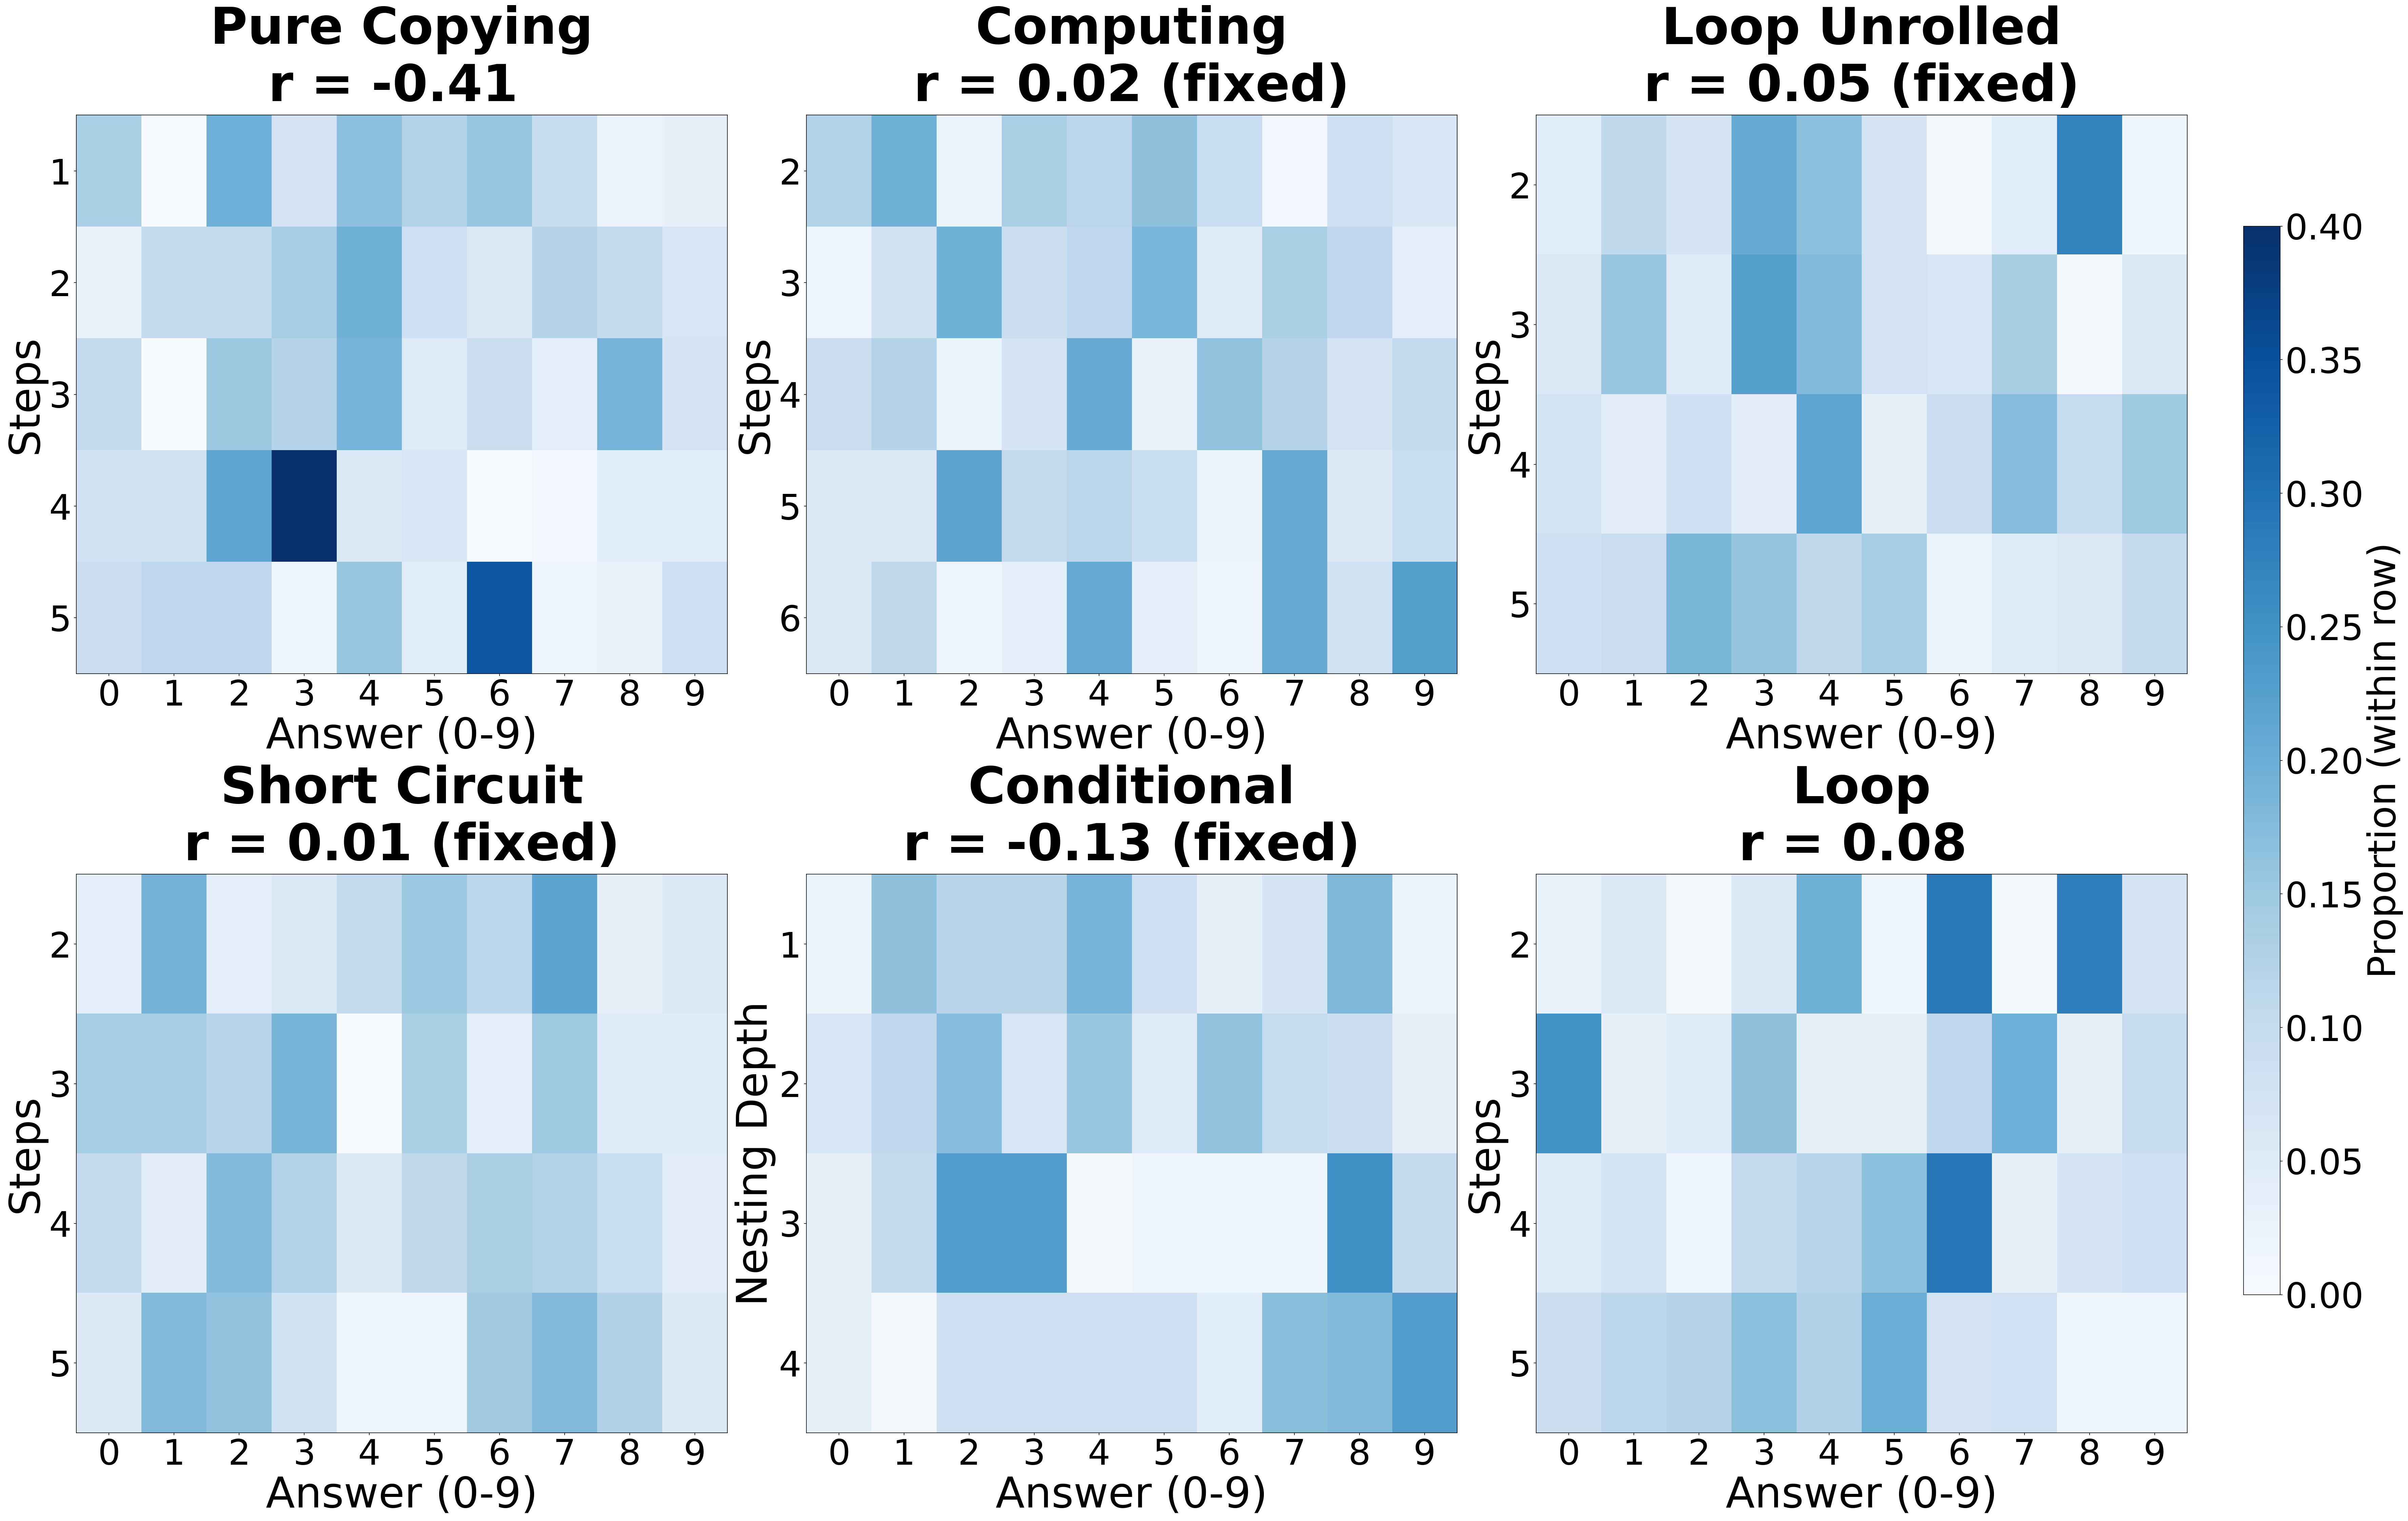
\includegraphics[width=\columnwidth]{figures/appendix/B_answer_distribution.png}
\caption{Answer distributions across control variables for all six tasks. Low Pearson correlations ($|r| < 0.15$ for debiased tasks) suggest that, after debiasing, difficulty parameters are not strongly associated with answer values.}
\label{fig:answer_dist}
\end{figure}


% Appendix C: Diagnostic Framework Details (includes C.1 Probing + C.2 CSD)
% Appendix C: Diagnostic Framework Details
% 包含 Probing 训练细节 (C.1) 和 CSD 实现细节 (C.2)

\section{Diagnostic Framework Details}
\label{app:diagnostic_framework_details}

% 本节汇总 dual diagnostic framework 的完整实现细节，补充正文 §2 中因篇幅省略的技术信息。

% Appendix B: Linear Probing Training Details

\section{Linear Probing Training Details}
\label{app:probing}

This appendix details the training procedure for the linear probing diagnostic $\Phi_{\mathrm{P}}^\ell$ introduced in \cref{sec:method}.

% ------------------------------------------------------------------
\subsection{Hidden State Extraction}
\label{app:subsec:probing_extraction}

For each task instance with source prompt $S = [C;\, Q]$, we perform a single forward pass through the target model $\mathcal{M}$ and extract the hidden state $\mathbf{h}^\ell \in \mathbb{R}^d$ at the \textbf{last token position} of every layer $\ell \in \{0, 1, \dots, L{-}1\}$. Due to the causal attention mask, the last token position aggregates information from all preceding tokens, making it the natural locus for probing what the model ``knows'' at each layer.

Each hidden state $\mathbf{h}^\ell$ is paired with a label $t^* \in \mathcal{T} = \{0, 1, \dots, 9, \bar{d}\}$, where $t^*$ is the ground-truth digit and $\bar{d}$ is never used as a ground-truth label---it exists only as a prediction target (see below).

% ------------------------------------------------------------------
\subsection{11-Class Classification Setup}
\label{app:subsec:probing_classes}

A standard probing setup for this benchmark would use 10-class classification over $\mathcal{D} = \{0, 1, \dots, 9\}$. We extend this to \textbf{11 classes} by introducing the residual class $\bar{d}$, which aggregates all non-digit tokens into a single category.

\paragraph{Training label construction.} Ground-truth labels are always digit classes ($t^* \in \{0, \dots, 9\}$). To construct training samples for the $\bar{d}$ class, we include hidden states from layers where the model's final output token (via standard forward pass) is a non-digit token. This ensures the probe learns to distinguish between ``the representation points toward a digit'' and ``the representation has not yet consolidated toward any digit answer.''

\paragraph{Rationale for $\bar{d}$.} The residual class serves as an \emph{error sink}: if $\arg\max \Phi_{\mathrm{P}}^\ell(\mathbf{h}^\ell) = \bar{d}$, the probe indicates that no digit is yet linearly separable in the activation space---the information is either absent or encoded in a format that a linear classifier cannot access. This gives the probing diagnostic a three-valued interpretation at each layer: (1)~correct digit, (2)~wrong digit, (3)~not yet a digit. Without $\bar{d}$, the probe would be forced to assign probability mass to some digit even when the representation carries no digit-relevant signal, inflating false positives in early layers.

% ------------------------------------------------------------------
\subsection{Per-Layer Classifier Training}
\label{app:subsec:probing_training}

We train \textbf{one independent classifier per layer} $\ell$, denoted $\Phi_{\mathrm{P}}^\ell$. Each classifier is a logistic regression model (multinomial, L2-regularized):
%
\begin{equation}
\Phi_{\mathrm{P}}^\ell(\mathbf{h}^\ell) = \mathrm{softmax}(W^\ell \mathbf{h}^\ell + \mathbf{b}^\ell)
\end{equation}
%
where $W^\ell \in \mathbb{R}^{11 \times d}$ and $\mathbf{b}^\ell \in \mathbb{R}^{11}$.

\paragraph{Implementation.} We use \texttt{sklearn.linear\_model.LogisticRegression} with the configuration in \cref{tab:probe_hyperparams}.

\begin{table}[h]
\centering
\resizebox{\columnwidth}{!}{%
\begin{tabular}{lll}
\toprule
\textbf{Hyperparameter} & \textbf{Value} & \textbf{Rationale} \\
\midrule
Solver        & \texttt{lbfgs}       & Standard for multinomial logistic regression \\
Regularization & L2, $C = 1.0$       & Prevents overfitting on high-dim.\ $\mathbf{h}^\ell$ \\
Max iterations & 1000                & Ensures convergence across all layers \\
Multi-class   & \texttt{multinomial}  & Joint optimization over all 11 classes \\
\bottomrule
\end{tabular}%
}
\caption{Probing classifier hyperparameters.}
\label{tab:probe_hyperparams}
\end{table}

\paragraph{Why logistic regression?} The choice of a linear classifier is deliberate and methodologically motivated. A linear probe tests whether the target information is \textbf{linearly separable} in the representation space---the weakest geometric condition for information presence. Using a more powerful classifier (e.g., MLP) would conflate ``the information exists'' with ``a nonlinear transformation can extract it,'' weakening the interpretive value of the necessary condition that probing is designed to establish. This follows established practice in representation probing \citep{belinkov2022probing, hewitt2019designing}.

% ------------------------------------------------------------------
\subsection{Train/Test Split}
\label{app:subsec:probing_split}

For each task family, the dataset is split into training and test sets. The probing classifier is trained on the training split and evaluated on the held-out test split. Importantly, the \textbf{same test split} is used for both probing ($\Phi_{\mathrm{P}}^\ell$) and activation verbalization ($\Phi_{\mathrm{C}}^\ell$), ensuring that the two diagnostics are evaluated on identical instances and their layer-wise agreement/disagreement is computed on matched samples.

% ------------------------------------------------------------------
\subsection{Evaluation Metrics}
\label{app:subsec:probing_eval}

For each layer $\ell$ and each test instance, we record:
\begin{itemize}
    \item $\hat{t}_{\mathrm{P}}^\ell = \arg\max \Phi_{\mathrm{P}}^\ell(\mathbf{h}^\ell)$: the probe's predicted class.
    \item Whether $\hat{t}_{\mathrm{P}}^\ell = t^*$ (correct), $\hat{t}_{\mathrm{P}}^\ell \in \mathcal{D} \setminus \{t^*\}$ (wrong digit), or $\hat{t}_{\mathrm{P}}^\ell = \bar{d}$ (non-digit).
\end{itemize}

The \textbf{First Probing Correct Layer (FPCL)} is defined as:
%
\begin{equation}
\mathrm{FPCL}(S) = \min \{ \ell \mid \hat{t}_{\mathrm{P}}^\ell = t^* \}
\end{equation}

The \textbf{Brewing Duration} $\Delta$ is the gap between FPCL and the First Correct Layer of CSD:
%
\begin{equation}
\Delta(S) = \mathrm{FCL}(S) - \mathrm{FPCL}(S)
\end{equation}

$\Delta > 0$ indicates that the information exists in the representation (the probe can read it) before the model's own decoding pathway can access it---the hallmark of \textbf{Information Brewing}.

% Appendix C.2: CSD Implementation Details

\subsection{CSD Implementation Details}
\label{app:subsec:csd_implementation}

% 详细描述 Context-Stripped Decoding 的实现：baseline subtraction 操作流程、target prompt 构造方式、
% 以及面向不熟悉 Patchscopes 的读者的背景补充。
% 预期效果：读者无需阅读 Patchscopes 原文即可理解 CSD 的完整操作。

This section provides a self-contained description of the Context-Stripped Decoding (CSD) procedure, so that readers unfamiliar with Patchscopes \citep{ghandeharioun2024patchscopes} can reproduce the method without consulting the original paper.
The formal definition is given in \cref{eq:csd}; here we unpack each step.

\paragraph{Step 1: Target prompt construction.}
Each code-understanding sample consists of a code context $C$ (the program) and a question suffix $Q$ (e.g., \texttt{\# The value of x is "}).
The \emph{source prompt} is the full concatenation $S = [C;\, Q]$.
The \emph{target prompt} retains only the question suffix: $T = Q$, thereby stripping away all code context.
Because $T$ contains no information about the program, any correct answer decoded from $T$ must originate from the patched hidden state rather than from the surrounding context.

\paragraph{Step 2: Patching procedure.}
For a given layer $\ell \in \{0, \dots, L{-}1\}$, CSD proceeds as follows:
\begin{enumerate}
    \item Run the source prompt $S = [C;\, Q]$ through the full model. Extract the hidden state $\mathbf{h}^\ell_S$ at the last token position at layer $\ell$.
    \item Construct a separate forward pass with the target prompt $T = Q$. At layer $\ell$, replace the last-token hidden state in the target run with $\mathbf{h}^\ell_S$ from the source run:
    \begin{equation}
    \label{eq:csd_patch}
    \tilde{\mathbf{h}}^\ell_T \;\leftarrow\; \mathbf{h}^\ell_S.
    \end{equation}
    \item Continue the target forward pass from layer $\ell{+}1$ through layer $L{-}1$, applying the remaining transformer blocks $F_{\ell+1}, \dots, F_{L-1}$, followed by LayerNorm and the unembedding matrix $W_u$. Crucially, the attention context for all subsequent layers is restricted to $T$, not the original $S$.
\end{enumerate}
This yields patched logits $\mathbf{z}_{\mathrm{patch}}^\ell = W_u \circ \mathrm{LN} \circ F_{L-1} \circ \cdots \circ F_{\ell+1}(\tilde{\mathbf{h}}^\ell_T)$.

\paragraph{Step 3: Baseline subtraction.}
Running the target prompt $T$ alone (without any patching) produces a baseline logit vector $\mathbf{z}_b$, which captures the language prior induced by $T$.
For instance, the question suffix \texttt{\# The value of x is "} may assign non-trivial probability to certain digits even without any code context.
To isolate the contribution of the patched hidden state, we subtract this baseline:
\begin{equation}
\label{eq:csd_subtract}
\mathbf{z}_{\mathrm{CSD}}^\ell = \mathbf{z}_{\mathrm{patch}}^\ell - \mathbf{z}_b.
\end{equation}
Finally, we apply softmax and restrict the resulting distribution to the target token set $\mathcal{T} = \mathcal{D} \cup \{\bar{d}\}$, where $\mathcal{D} = \{0, 1, \dots, 9\}$ is the set of digit tokens and $\bar{d}$ is a residual class:
\begin{equation}
\label{eq:csd_distribution}
\Phi_{\mathrm{C}}^\ell(\mathbf{h}^\ell)[t] = \frac{\exp(\mathbf{z}_{\mathrm{CSD}}^\ell[t])}{\sum_{t' \in \mathcal{T}} \exp(\mathbf{z}_{\mathrm{CSD}}^\ell[t'])}, \quad t \in \mathcal{T}.
\end{equation}
This recovers the CSD distribution defined in \cref{eq:csd}.

\paragraph{Step 4: Practical considerations.}
Several implementation details are worth noting:

\begin{itemize}
    \item \textbf{Layer-wise independence.} Patching is performed at each layer $\ell \in \{0, \dots, L{-}1\}$ independently.
    Each layer produces its own CSD distribution $\Phi_{\mathrm{C}}^\ell$; there is no cross-layer interaction between patching runs.

    \item \textbf{Baseline reuse.} The baseline logit $\mathbf{z}_b$ depends only on the target prompt $T$ and is therefore identical across all layers for a given sample.
    We compute $\mathbf{z}_b$ once and reuse it for all $L$ patching runs, reducing the total number of forward passes from $2L$ to $L{+}1$ per sample.

    \item \textbf{Hook-based implementation.} In practice, we implement the hidden-state replacement using PyTorch forward hooks.
    A hook registered at layer $\ell$ intercepts the target run's hidden state and overwrites the last-token position with $\mathbf{h}^\ell_S$.
    This avoids modifying the model architecture and allows patching at arbitrary layers without rerunning earlier layers of the target pass.

    \item \textbf{Positional encoding.} Because the source prompt $S$ and target prompt $T$ have different lengths, the absolute position index of the last token differs between the two runs.
    Following \citet{ghandeharioun2024patchscopes}, we do not adjust positional encodings when patching; the injected hidden state retains the positional information from the source run.
    In the Qwen2.5-Coder architecture, which uses Rotary Position Embeddings (RoPE), this means the patched state carries the source-side rotary phase.
    We verified empirically that this does not degrade the diagnostic's discriminative power for our single-token prediction task.
\end{itemize}



% Appendix D: Outcome Definition and Statistics
% Appendix D: Outcome Definition and Statistics

\section{Outcome Definition and Statistics}
\label{app:outcome_distribution_statistics}

% 本节提供四类 resolution outcome 的完整统计数据，补充正文 §3 中的汇总数字。

\subsection{Outcome Distributions by Task and Model}
\label{app:subsec:outcome_results_by_task}

% 主要模型 × 六任务的 Resolved / Overprocessed / Misresolved / Unresolved 完整表格。
% 预期效果：读者可查阅任意模型-任务组合的 outcome 分布。

% TODO: 插入 outcome 分布表格

\subsection{FPCL and FJC Layer Positions}
\label{app:subsec:fpcl_fjc_layer_positions}

% 各任务和模型的归一化 FPCL、FJC 出现层位统计（均值、标准差、分布图）。
% 预期效果：量化 brewing 的起止位置在不同条件下的变化。

% TODO: 插入 FPCL/FJC 层位统计

\subsection{FJC Existence and Final Correctness}
\label{app:subsec:fjc_correctness_correlation}

% FJC 是否存在与最终输出正确率之间的强相关性数据。
% 预期效果：为正文中 "FJC = ∅ 几乎等价于做错" 的 claim 提供完整支撑。

% TODO: 插入 FJC-correctness 相关性数据


% Appendix E: Causal Validation Experiments
% Appendix E: Causal Validation Experiments

\section{Causal Validation Experiments}
\label{app:causal_validation_details}

% 本节提供正文 §3.1 三组因果实验的完整设置、层位扫描结果与失败案例。

\subsection{Activation Patching at FJC}
\label{app:subsec:activation_patching_fjc}

% 详细实验设置：task-matched sample 配对策略、patching 操作流程。
% 层位扫描：不同层的 answer-flip rate 曲线，展示 FJC 的因果特权性。
% 预期效果：读者可看到 FJC 层 flip rate 相对其他层的显著优势。

% TODO: 插入 patching 实验细节与层位扫描图

\subsection{Layer Skipping for Overprocessed}
\label{app:subsec:layer_skipping_overprocessed}

% 跳过 FJC 之后尾部层的具体操作与解码方式。
% Resolved vs. Overprocessed 上的效果对比，展示 outcome 特异性。
% 预期效果：证明 Overprocessed 确实是"先对后错"，跳过后期层可恢复。

% TODO: 插入 layer skipping 实验结果

\subsection{Late-Layer Hidden-State Sparsity in Overprocessed Samples}
\label{app:subsec:late_layer_sparsity_overprocessed}

As a descriptive complement to the layer-skipping intervention, we also examine whether Overprocessed samples exhibit a distinct late-layer representation geometry.
Using the full Qwen2.5-Coder-7B Computing dataset ($N=1800$), we aggregate two standard sparsity measures from the last-token hidden state at every layer: the Gini index and Hoyer sparsity.

\cref{fig:app:hidden_state_sparsity} shows that the two measures peak at different depths.
The Gini index rises earlier and reaches its maximum around the middle-to-late layers, whereas Hoyer sparsity stays relatively moderate until the final block and then spikes sharply near layer 26.
This temporal separation is consistent with a two-stage picture in which representations first become more concentrated and later undergo a stronger sparsification during the final decoding-relevant phase.

To test whether this late sparsification is specifically associated with degradation after internal success, we compare Overprocessed and non-Overprocessed valid samples at layers 24--27.
As shown in \cref{fig:app:hoyer_ot_vs_nonot}, Overprocessed samples have consistently higher Hoyer sparsity at all four late layers, with the largest gap at layer 26 where global Hoyer also peaks.
Because this analysis is observational rather than interventional, we do not treat sparsity as causal evidence.
Instead, we view it as a representation-level correlate of overprocessing: once a correct answer has become jointly available, the final degradation phase is accompanied by a measurable compression-like shift in hidden-state geometry.

\begin{figure*}[t]
\centering
\begin{subfigure}[t]{0.58\textwidth}
    \centering
    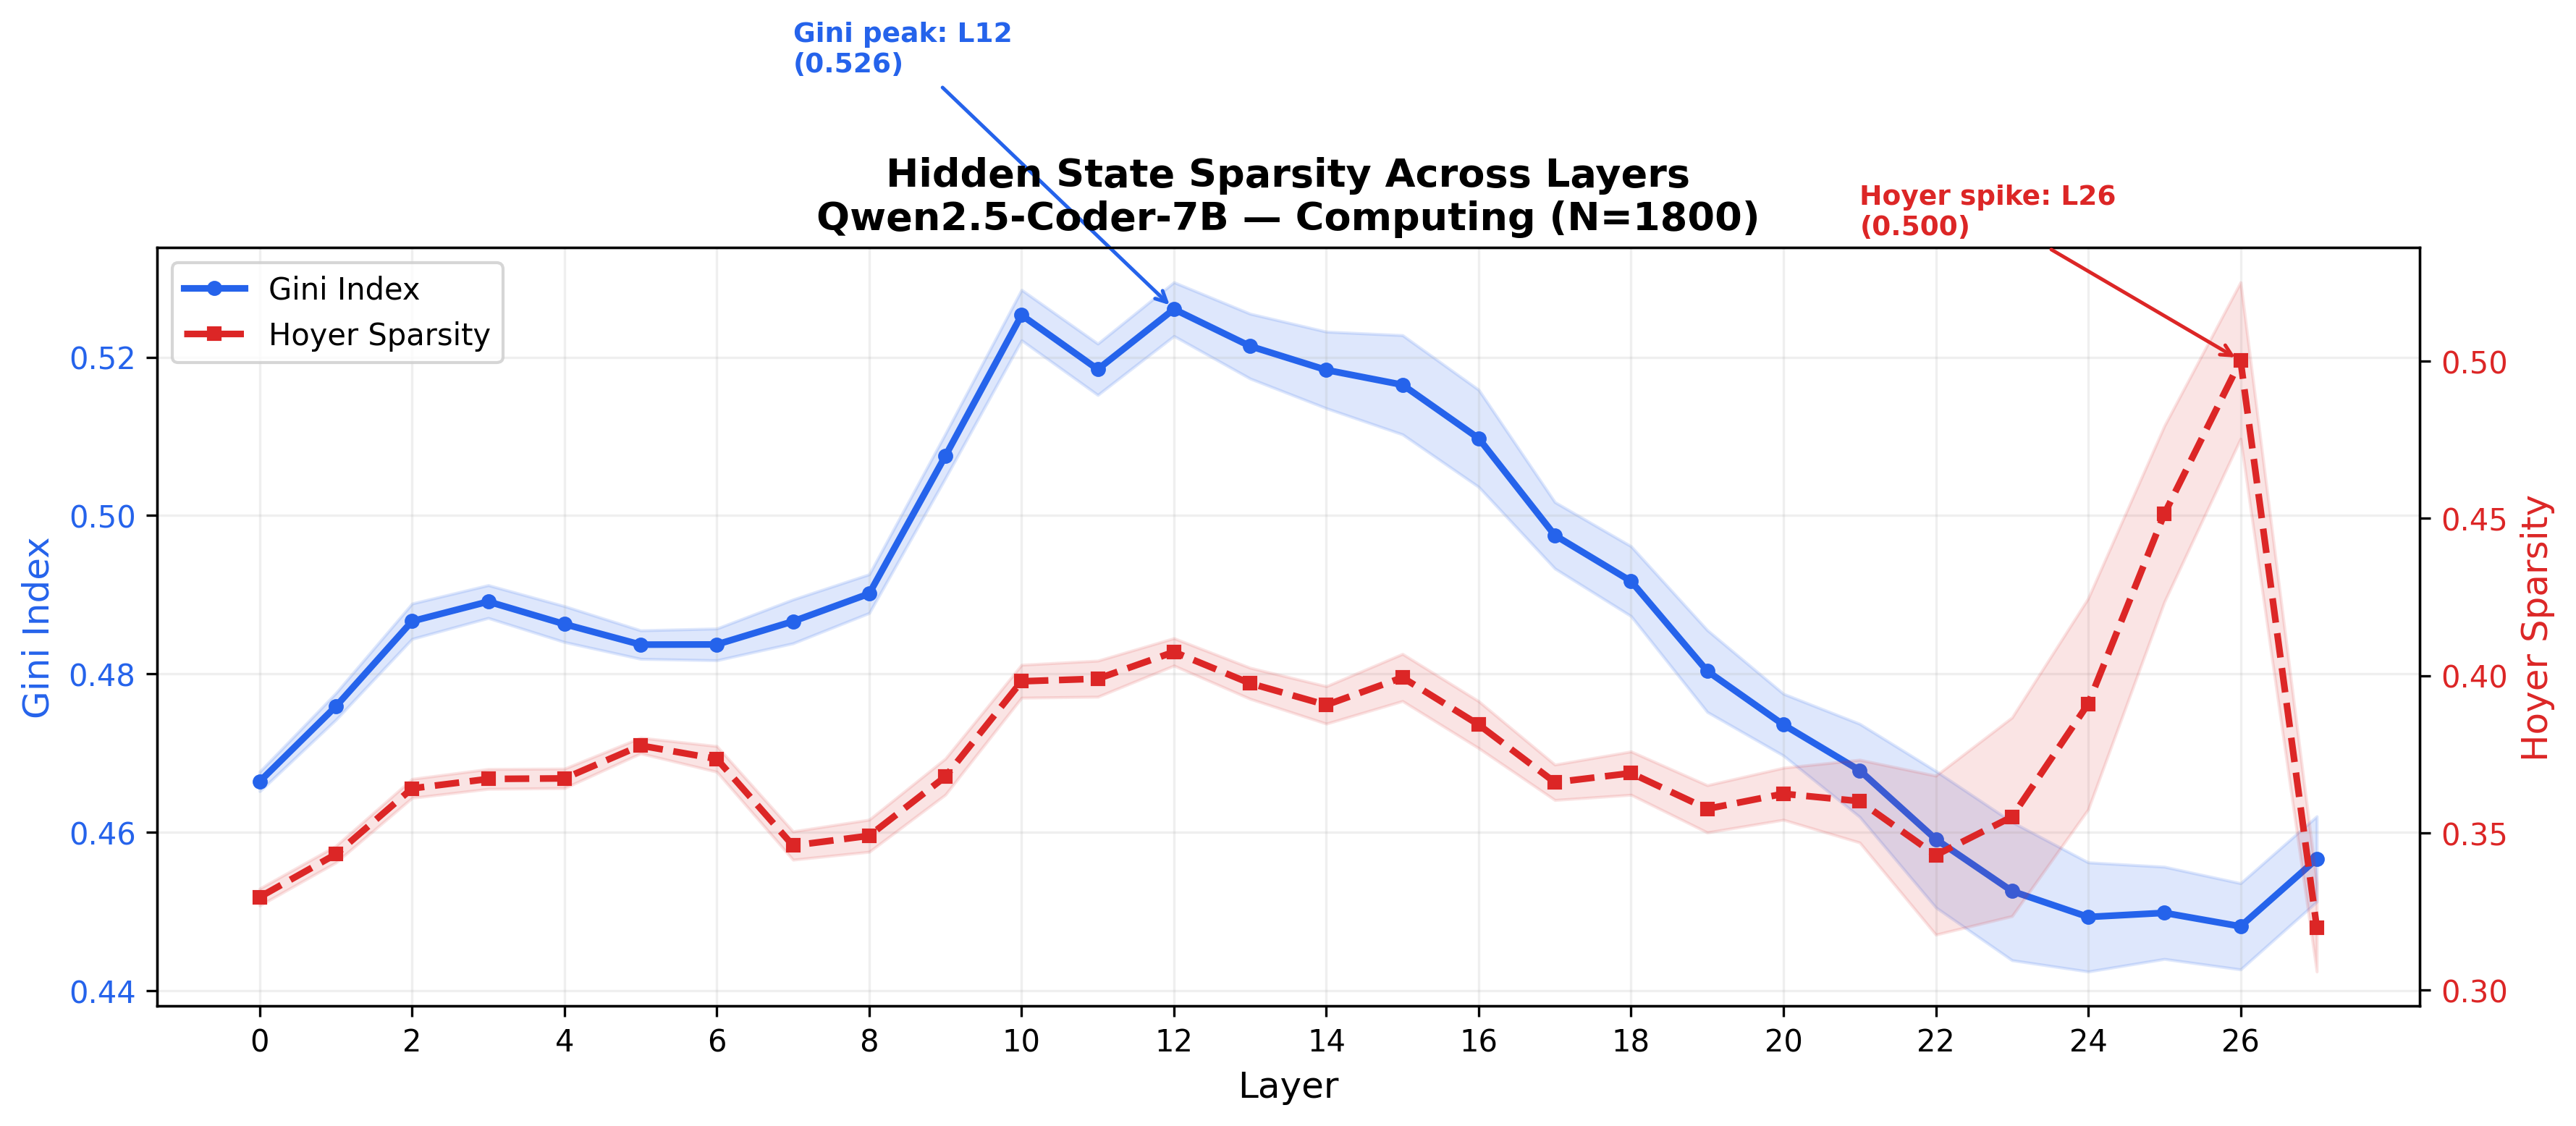
\includegraphics[width=\textwidth]{figures/appendix/causal_hidden_state_sparsity.png}
    \caption{Global layer-wise Gini and Hoyer curves on the full Qwen2.5-Coder-7B Computing set.}
    \label{fig:app:hidden_state_sparsity}
\end{subfigure}
\hfill
\begin{subfigure}[t]{0.38\textwidth}
    \centering
    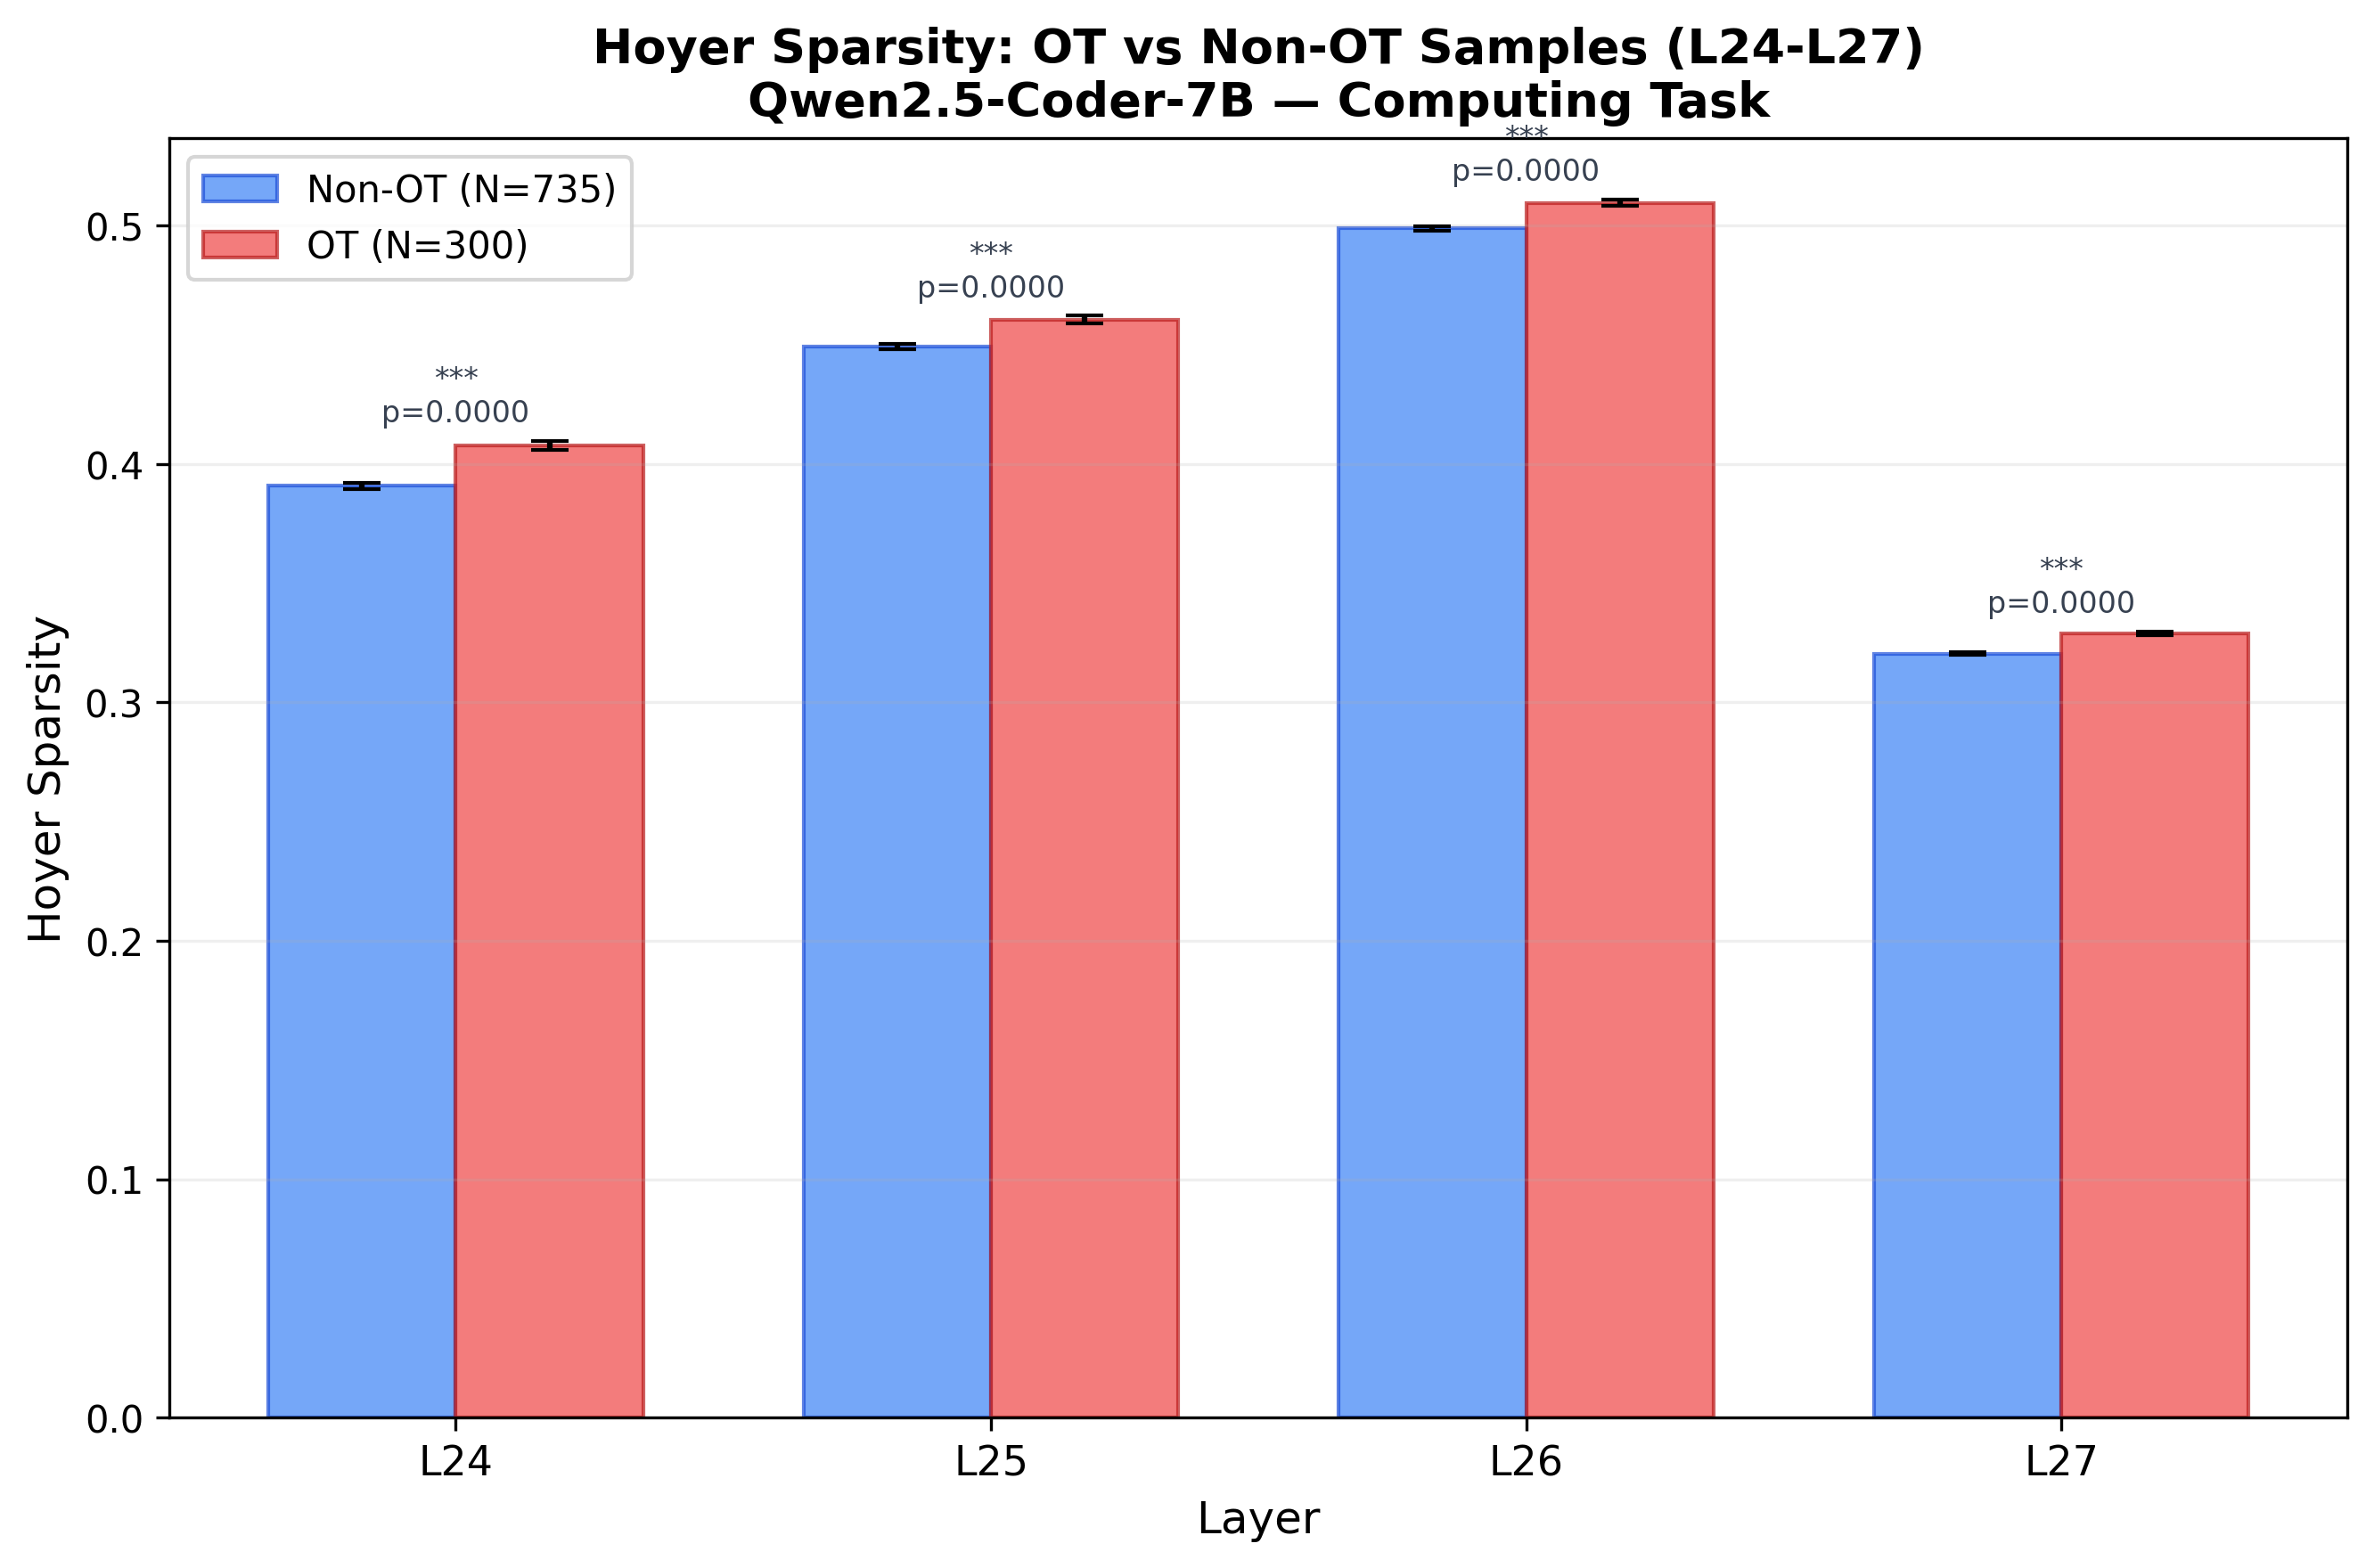
\includegraphics[width=\textwidth]{figures/appendix/causal_hoyer_ot_vs_nonot.png}
    \caption{Late-layer Hoyer sparsity for Overprocessed vs.\ non-Overprocessed valid samples.}
    \label{fig:app:hoyer_ot_vs_nonot}
\end{subfigure}
\caption{Late-layer hidden-state sparsity as a descriptive correlate of Overprocessed trajectories in the anchor setting (Qwen2.5-Coder-7B, Computing).}
\label{fig:app:overprocessed_sparsity}
\end{figure*}

\subsection{Re-injection for Unresolved}
\label{app:subsec:reinjection_unresolved}

% 重注入流程：如何将后期 hidden state 注入新的前向传播以提供额外有效深度。
% Rescue rate 计算与结果。
% 预期效果：证明 Unresolved 多数是"没算完"而非"根本不会"。

% TODO: 插入 re-injection 实验结果

\subsection{Failure Cases}
\label{app:subsec:causal_failure_cases}

% 三组因果实验中干预无效的典型案例分析。
% 预期效果：诚实地展示方法边界，增强可信度。

% TODO: 插入失败案例分析


% Appendix F: GT-free Outcome Signals
% Appendix F: GT-free Outcome Signals

\section{GT-free Outcome Signals}
\label{app:ground_truth_free_discrimination}

% 本节展示如何仅用模型自身的输出分布信号（无需 ground truth）区分四类 outcome。
% 对应之前 part2 的实验结果。

\subsection{Signal Definitions}
\label{app:subsec:gtfree_signal_definitions}

% 三个 GT-free 信号的形式化定义：
%   (1) CSD entropy H_C^ℓ
%   (2) Entropy 下降速率 dH_C/dℓ
%   (3) Probe-CSD agreement A^ℓ
% 预期效果：读者可精确理解每个信号的计算方式。

% TODO: 插入信号定义

\subsection{Outcome-Specific Signal Characteristics}
\label{app:subsec:gtfree_outcome_signatures}

% 四类 outcome 在三个信号空间中的分布可视化。
% 区分方案（阈值或分类器）及其性能。
% 预期效果：直观展示 GT-free 信号确实能区分四类 outcome。

% TODO: 插入信号特征可视化与区分方案


% Appendix G: Cross-Task Analysis
% Appendix G: Cross-Task Analysis

\section{Cross-Task Analysis}
\label{app:cross_task_analysis}

This appendix provides the complete cross-task data underlying the comparisons in \S4.
All results use Qwen2.5-Coder-7B ($L{=}28$) unless stated otherwise.

%% ========== G.1 ==========
\subsection{Outcome Fingerprints: Full Data}
\label{app:subsec:outcome_fingerprints_full}

\cref{tab:app:outcome_fingerprint_full} reports the aggregate outcome distributions with per-task commentary on dominant failure modes.

\begin{table*}[t]
\centering
\caption{Full outcome fingerprints for Qwen2.5-Coder-7B across all six task families, with per-task commentary on failure characteristics.
Res.\ = Resolved, OT = Overprocessed, MR = Misresolved, UR = Unresolved.}
\label{tab:app:outcome_fingerprint_full}
\resizebox{\textwidth}{!}{%
\begin{tabular}{lrccccp{5.8cm}}
\toprule
Task & $N$ & Res.\% & OT\% & MR\% & UR\% & Commentary \\
\midrule
Pure Copying & 200 & 79.0 & 21.0 & 0.0 & 0.0 &
No MR or UR: the model always converges, but 21\% of samples are overprocessed---late layers corrupt a once-correct trace. \\
Computing & 207 & 33.5 & 45.9 & 12.4 & 8.1 &
Uniquely difficult: all four outcomes present in substantial proportions. Overprocessed dominates (45.9\%), yet it is the only task with notable MR (12.4\%) and UR (8.1\%), indicating qualitatively different failure modes. \\
Loop Unrolled & 298 & 89.3 & 8.1 & 2.7 & 0.0 &
Near-zero UR: the model always forms a convergence point. Residual MR (2.7\%) arises at high iteration counts. \\
Loop & 408 & 84.8 & 10.8 & 3.9 & 0.5 &
Similar to Loop Unrolled but with slightly elevated OT and a small UR fraction (0.5\%), syntactic loop structure adds marginal processing difficulty. \\
Conditional & 542 & 82.7 & 11.4 & 4.4 & 1.5 &
OT and MR rise together at high nesting depths; UR appears only at depth 3, indicating that deeply nested branches occasionally prevent convergence entirely. \\
Short-circuit & 346 & 86.1 & 10.4 & 3.5 & 0.0 &
Zero UR across all difficulty levels: the model always commits to an answer. Failures are exclusively OT or MR, consistent with the binary nature of short-circuit evaluation. \\
\midrule
Weighted avg. & 2001 & 79.2 & 15.1 & 4.3 & 1.3 & --- \\
\bottomrule
\end{tabular}%
}
\end{table*}

\paragraph{Computing as the sole four-way outlier.}
Computing is the only task where all four outcomes appear in substantial proportions.
The remaining five tasks share a common signature: Resolved $>$ 79\%, Overprocessed as the primary failure mode (8--21\%), and Misresolved and Unresolved together below 6\%.


%% ========== G.2 ==========
\subsection{Computing Density Sweep}
\label{app:subsec:computing_density_sweep}

The Computing task has two orthogonal difficulty axes: compute density $\rho \in \{0, 0.5, 1.0\}$ (fraction of steps requiring arithmetic) and chain length (steps $\in \{2,3,4,5\}$).
We sweep each independently.

\paragraph{Compute density ($\rho$) sweep.}

\cref{tab:app:rho_sweep} reports outcome distributions and mean brewing duration as $\rho$ increases.

\begin{table}[H]
\centering
\caption{Outcome distribution and mean brewing duration ($\Delta_{\mathrm{brew}}$) as a function of compute density $\rho$ for the Computing task (Qwen2.5-Coder-7B, pooled over all chain lengths).}
\label{tab:app:rho_sweep}
\resizebox{\columnwidth}{!}{%
\begin{tabular}{crccccc}
\toprule
$\rho$ & $N$ & Res.\% & OT\% & MR\% & UR\% & $\overline{\Delta}_{\mathrm{brew}}$ \\
\midrule
0   & 525 & 40.0 & 45.1 & 12.2 & 2.7 & 17.9 \\
0.5 & 309 & 19.7 & 23.6 & 30.1 & 26.5 & 13.4 \\
1.0 & 201 & 16.4 & 17.9 & 26.9 & 38.8 & 8.6 \\
\bottomrule
\end{tabular}%
}
\end{table}

\paragraph{Failure mode shift with arithmetic density.}
Even at $\rho{=}0$, the Resolved rate is lower than structurally similar control-flow tasks; multi-hop variable tracking itself is a bottleneck.
As $\rho$ increases, the failure character shifts: OT dominates at $\rho{=}0$, whereas MR and UR grow disproportionately at $\rho{=}1.0$, indicating that arithmetic demands \textbf{change the failure mechanism} from late-layer corruption to inability to reach the correct answer.
The brewing duration $\overline{\Delta}_{\mathrm{brew}}$ also contracts, consistent with the probe detecting partial (but incorrect) information earlier.

\paragraph{Chain length (steps) sweep.}

\cref{tab:app:step_sweep} isolates the effect of chain length.

\begin{table}[H]
\centering
\caption{Outcome distribution and layer-position statistics as a function of chain length (steps) for the Computing task (Qwen2.5-Coder-7B, pooled over all $\rho$).}
\label{tab:app:step_sweep}
\resizebox{\columnwidth}{!}{%
\begin{tabular}{crcccccc}
\toprule
Steps & $N$ & Res.\% & OT\% & MR\% & UR\% & $\overline{\mathrm{FPCL}}$ & $\overline{\mathrm{FJC}}$ \\
\midrule
2 & 260 & 48 & 38 & 8 & 6 & 7 & 20 \\
3 & 260 & 35 & 40 & 14 & 11 & 9 & 21 \\
4 & 260 & 24 & 42 & 18 & 16 & 10 & 21 \\
5 & 260 & 18 & 44 & 20 & 18 & 11 & 21 \\
\bottomrule
\end{tabular}%
}
\end{table}

\paragraph{Chain length as independent difficulty factor.}
Increasing chain length degrades outcomes even within fixed $\rho$ strata, demonstrating that sequential depth is an independent difficulty factor.
FPCL shifts later with longer chains while FJC remains stable, compressing the brewing window $\Delta_{\mathrm{brew}}$---mirroring the $\rho$-sweep pattern.


%% ========== G.3 ==========
\subsection{Per-Difficulty-Level Breakdown}
\label{app:subsec:per_difficulty_breakdown}

\cref{tab:app:per_difficulty_outcome} provides the complete per-difficulty-level outcome breakdown for all six task families.

\begin{table*}[t]
\centering
\caption{Per-difficulty-level outcome distributions for all six task families on Qwen2.5-Coder-7B.
Difficulty parameter varies by task: \emph{steps} for Copying and Computing (the latter at $\rho{=}1.0$), \emph{depth} for Conditional, \emph{num\_conditions} for Short-circuit, and \emph{iteration} for Loop and Loop Unrolled.}
\label{tab:app:per_difficulty_outcome}
\resizebox{\textwidth}{!}{%
\begin{tabular}{llrcccc}
\toprule
Task & Difficulty & $N$ & Res.\% & OT\% & MR\% & UR\% \\
\midrule
\multirow{5}{*}{Copying}
 & steps = 1 & 40 & 95.0 & 5.0 & 0.0 & 0.0 \\
 & steps = 2 & 40 & 87.5 & 12.5 & 0.0 & 0.0 \\
 & steps = 3 & 40 & 77.5 & 22.5 & 0.0 & 0.0 \\
 & steps = 4 & 40 & 72.5 & 27.5 & 0.0 & 0.0 \\
 & steps = 5 & 40 & 62.5 & 37.5 & 0.0 & 0.0 \\
\midrule
\multirow{4}{*}{Computing ($\rho{=}1.0$)}
 & steps = 2 & 51 & 33.3 & 23.5 & 17.6 & 25.5 \\
 & steps = 3 & 50 & 18.0 & 20.0 & 26.0 & 36.0 \\
 & steps = 4 & 50 & 10.0 & 16.0 & 30.0 & 44.0 \\
 & steps = 5 & 50 & 4.0 & 12.0 & 34.0 & 50.0 \\
\midrule
\multirow{3}{*}{Conditional}
 & depth = 1 & 196 & 98.0 & 2.0 & 0.0 & 0.0 \\
 & depth = 2 & 190 & 83.2 & 13.7 & 3.2 & 0.0 \\
 & depth = 3 & 156 & 62.8 & 20.5 & 11.5 & 5.1 \\
\midrule
\multirow{3}{*}{Short-circuit}
 & num\_cond = 1 & 72 & 100.0 & 0.0 & 0.0 & 0.0 \\
 & num\_cond = 2 & 134 & 83.6 & 10.4 & 6.0 & 0.0 \\
 & num\_cond = 3 & 140 & 81.4 & 15.7 & 2.9 & 0.0 \\
\midrule
\multirow{4}{*}{Loop}
 & iteration = 1 & 160 & 97.5 & 2.5 & 0.0 & 0.0 \\
 & iteration = 2 & 88 & 56.8 & 36.4 & 6.8 & 0.0 \\
 & iteration = 3 & 90 & 80.0 & 8.9 & 8.9 & 2.2 \\
 & iteration = 4 & 70 & 97.1 & 0.0 & 2.9 & 0.0 \\
\midrule
\multirow{4}{*}{Loop Unrolled}
 & iteration = 1 & 80 & 90.0 & 10.0 & 0.0 & 0.0 \\
 & iteration = 2 & 80 & 100.0 & 0.0 & 0.0 & 0.0 \\
 & iteration = 3 & 80 & 95.0 & 2.5 & 2.5 & 0.0 \\
 & iteration = 4 & 58 & 65.5 & 24.1 & 10.3 & 0.0 \\
\bottomrule
\end{tabular}%
}
\end{table*}

\paragraph{Per-task failure signatures across difficulty.}

\begin{itemize}
\item \textbf{Copying} exhibits OT as the sole failure mode at every difficulty level, with zero MR/UR---pure variable lookup always converges.

\item \textbf{Computing ($\rho{=}1.0$)} shows a steep Resolved decline with steps; by steps$\,{=}\,5$, MR and UR together exceed OT, indicating the model increasingly fails to reach the correct answer rather than losing it in late layers.

\item \textbf{Conditional} shows depth-dependent MR emergence: near-zero at depth 1, substantial at depth 3, suggesting nested branches introduce genuine resolution ambiguity.

\item \textbf{Short-circuit} maintains zero UR across all difficulty levels, consistent with the binary nature of the task.

\item \textbf{Loop vs.\ Loop Unrolled} differ in degradation shape: Loop exhibits a non-monotonic U-shaped pattern (dipping at iteration$\,{=}\,2$), while Loop Unrolled degrades more steeply at iteration$\,{=}\,4$, indicating that syntactic loop structure provides a processing scaffold that partially buffers against iteration-count difficulty.
\end{itemize}


%% ========== G.4 ==========
\subsection{Brewing Dynamics Comparison}
\label{app:subsec:brewing_dynamics_comparison}

\cref{tab:app:brewing_per_difficulty} reports brewing dynamics statistics per task and difficulty level.

\begin{table*}[t]
\centering
\caption{Brewing dynamics per task and difficulty level for Qwen2.5-Coder-7B.
FPCL and FJC are in layers ($L{=}28$ total); FJC exist.\ reports the fraction of samples for which an FJC was identified; $\Delta_{\mathrm{brew}} = \mathrm{FJC} - \mathrm{FPCL}$ is computed only over samples with both FPCL and FJC.}
\label{tab:app:brewing_per_difficulty}
\resizebox{\textwidth}{!}{%
\begin{tabular}{llcccc}
\toprule
Task & Difficulty & $\overline{\mathrm{FPCL}}$ & $\overline{\mathrm{FJC}}$ & FJC exist.\% & $\overline{\Delta}_{\mathrm{brew}}$ \\
\midrule
\multirow{5}{*}{Copying}
 & steps = 1 & 1.4 & 19.5 & 100 & 18.1 \\
 & steps = 2 & 1.6 & 19.7 & 100 & 18.1 \\
 & steps = 3 & 1.8 & 19.4 & 100 & 17.6 \\
 & steps = 4 & 1.7 & 19.8 & 100 & 18.1 \\
 & steps = 5 & 2.1 & 19.6 & 100 & 17.5 \\
\midrule
\multirow{4}{*}{Computing ($\rho{=}1.0$)}
 & steps = 2 & 7.8 & 20.6 & 57 & 12.8 \\
 & steps = 3 & 9.6 & 20.9 & 38 & 11.3 \\
 & steps = 4 & 10.8 & 20.7 & 26 & 9.9 \\
 & steps = 5 & 11.4 & 21.2 & 16 & 9.8 \\
\midrule
\multirow{3}{*}{Conditional}
 & depth = 1 & 6.4 & 19.3 & 100 & 12.9 \\
 & depth = 2 & 7.6 & 19.5 & 97 & 11.9 \\
 & depth = 3 & 8.3 & 19.4 & 83 & 11.1 \\
\midrule
\multirow{3}{*}{Short-circuit}
 & num\_cond = 1 & 3.4 & 19.3 & 100 & 15.9 \\
 & num\_cond = 2 & 4.1 & 19.5 & 94 & 15.4 \\
 & num\_cond = 3 & 4.6 & 19.8 & 97 & 15.2 \\
\midrule
\multirow{4}{*}{Loop}
 & iteration = 1 & 4.7 & 20.4 & 100 & 15.7 \\
 & iteration = 2 & 5.3 & 20.8 & 93 & 15.5 \\
 & iteration = 3 & 5.4 & 20.6 & 89 & 15.2 \\
 & iteration = 4 & 5.9 & 21.1 & 97 & 15.2 \\
\midrule
\multirow{4}{*}{Loop Unrolled}
 & iteration = 1 & 3.9 & 20.4 & 100 & 16.5 \\
 & iteration = 2 & 3.8 & 20.6 & 100 & 16.8 \\
 & iteration = 3 & 4.3 & 20.8 & 98 & 16.5 \\
 & iteration = 4 & 4.7 & 20.9 & 90 & 16.2 \\
\bottomrule
\end{tabular}%
}
\end{table*}

\paragraph{Stable scaffold, variable capability.}
Three patterns emerge:

\begin{enumerate}
\item \textbf{Positional stability of the brewing scaffold.}
Mean FPCL and FJC positions do not shift dramatically with difficulty across any task (e.g., Loop FPCL stays in layers 4--6, FJC in layers 19--22), indicating that the processing architecture is largely difficulty-independent.

\item \textbf{FJC existence rate as the primary difficulty-sensitive variable.}
What changes with difficulty is not \emph{where} the model processes information but \emph{whether} it reaches a convergence point. Declining FJC existence maps directly onto increased MR/UR outcomes, cleanly separating \emph{mechanism} (stable) from \emph{capability} (difficulty-dependent).

\item \textbf{Brewing duration compression under difficulty.}
In tasks where FPCL shifts later with difficulty (notably Computing), $\Delta_{\mathrm{brew}}$ compresses because FJC remains anchored, leaving less representational room for the correct answer to mature.
\end{enumerate}

\begin{figure}[t]
\centering
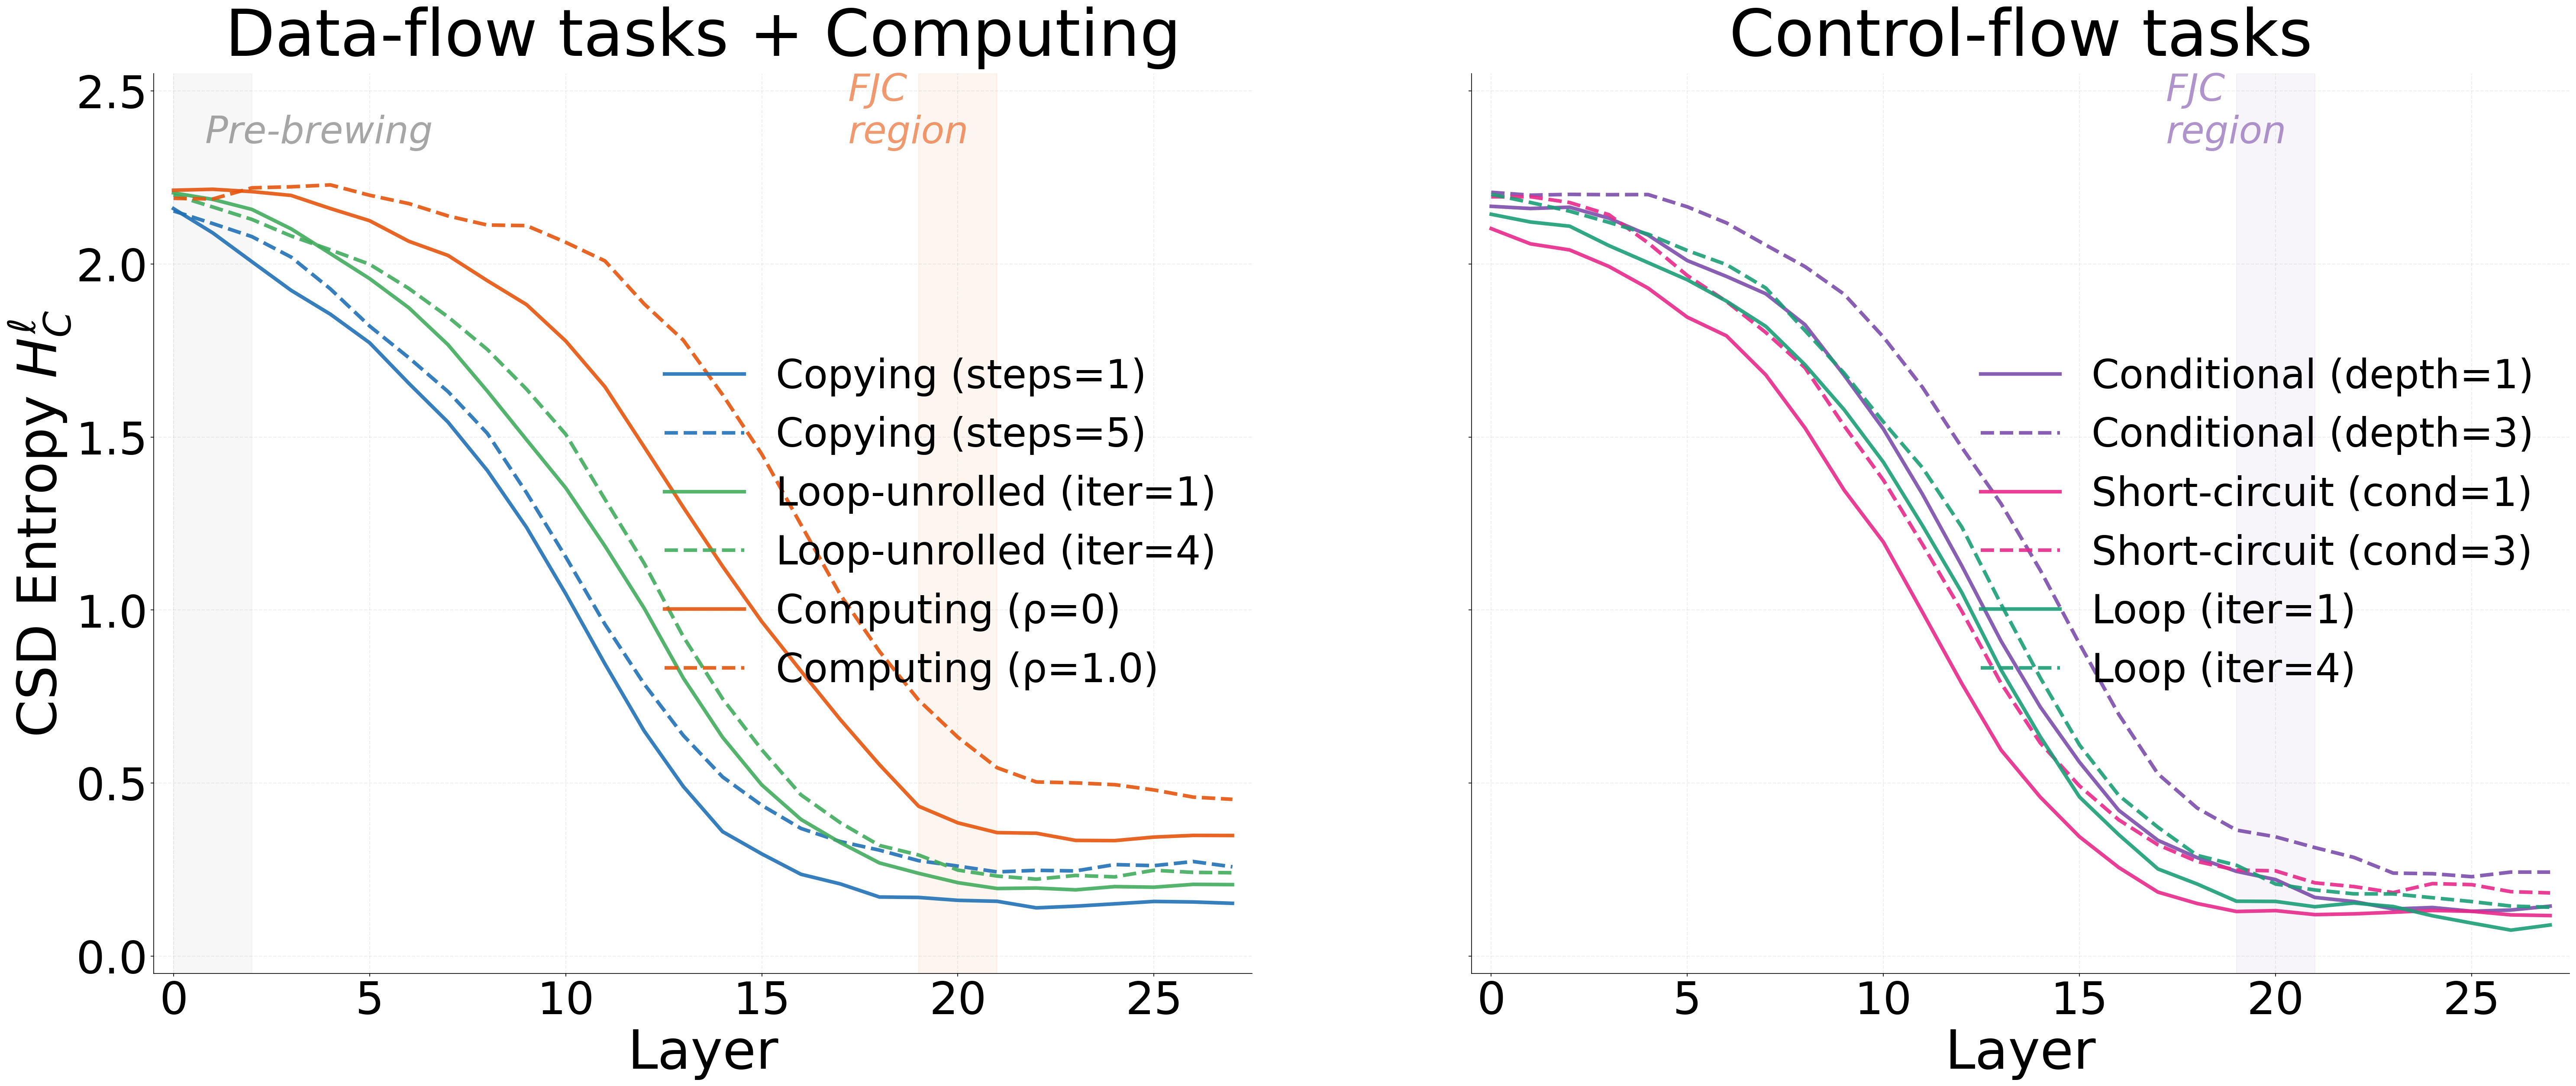
\includegraphics[width=\linewidth]{figures/appendix/G_brewing_dynamics_entropy.png}
\caption{Per-layer CSD entropy $H_C^\ell$ curves for each task at selected difficulty levels. The descent onset (related to FPCL) and convergence point (related to FJC) remain positionally stable; what varies is whether convergence is achieved.}
\label{fig:app:brewing_entropy}
\end{figure}

\begin{figure}[t]
\centering
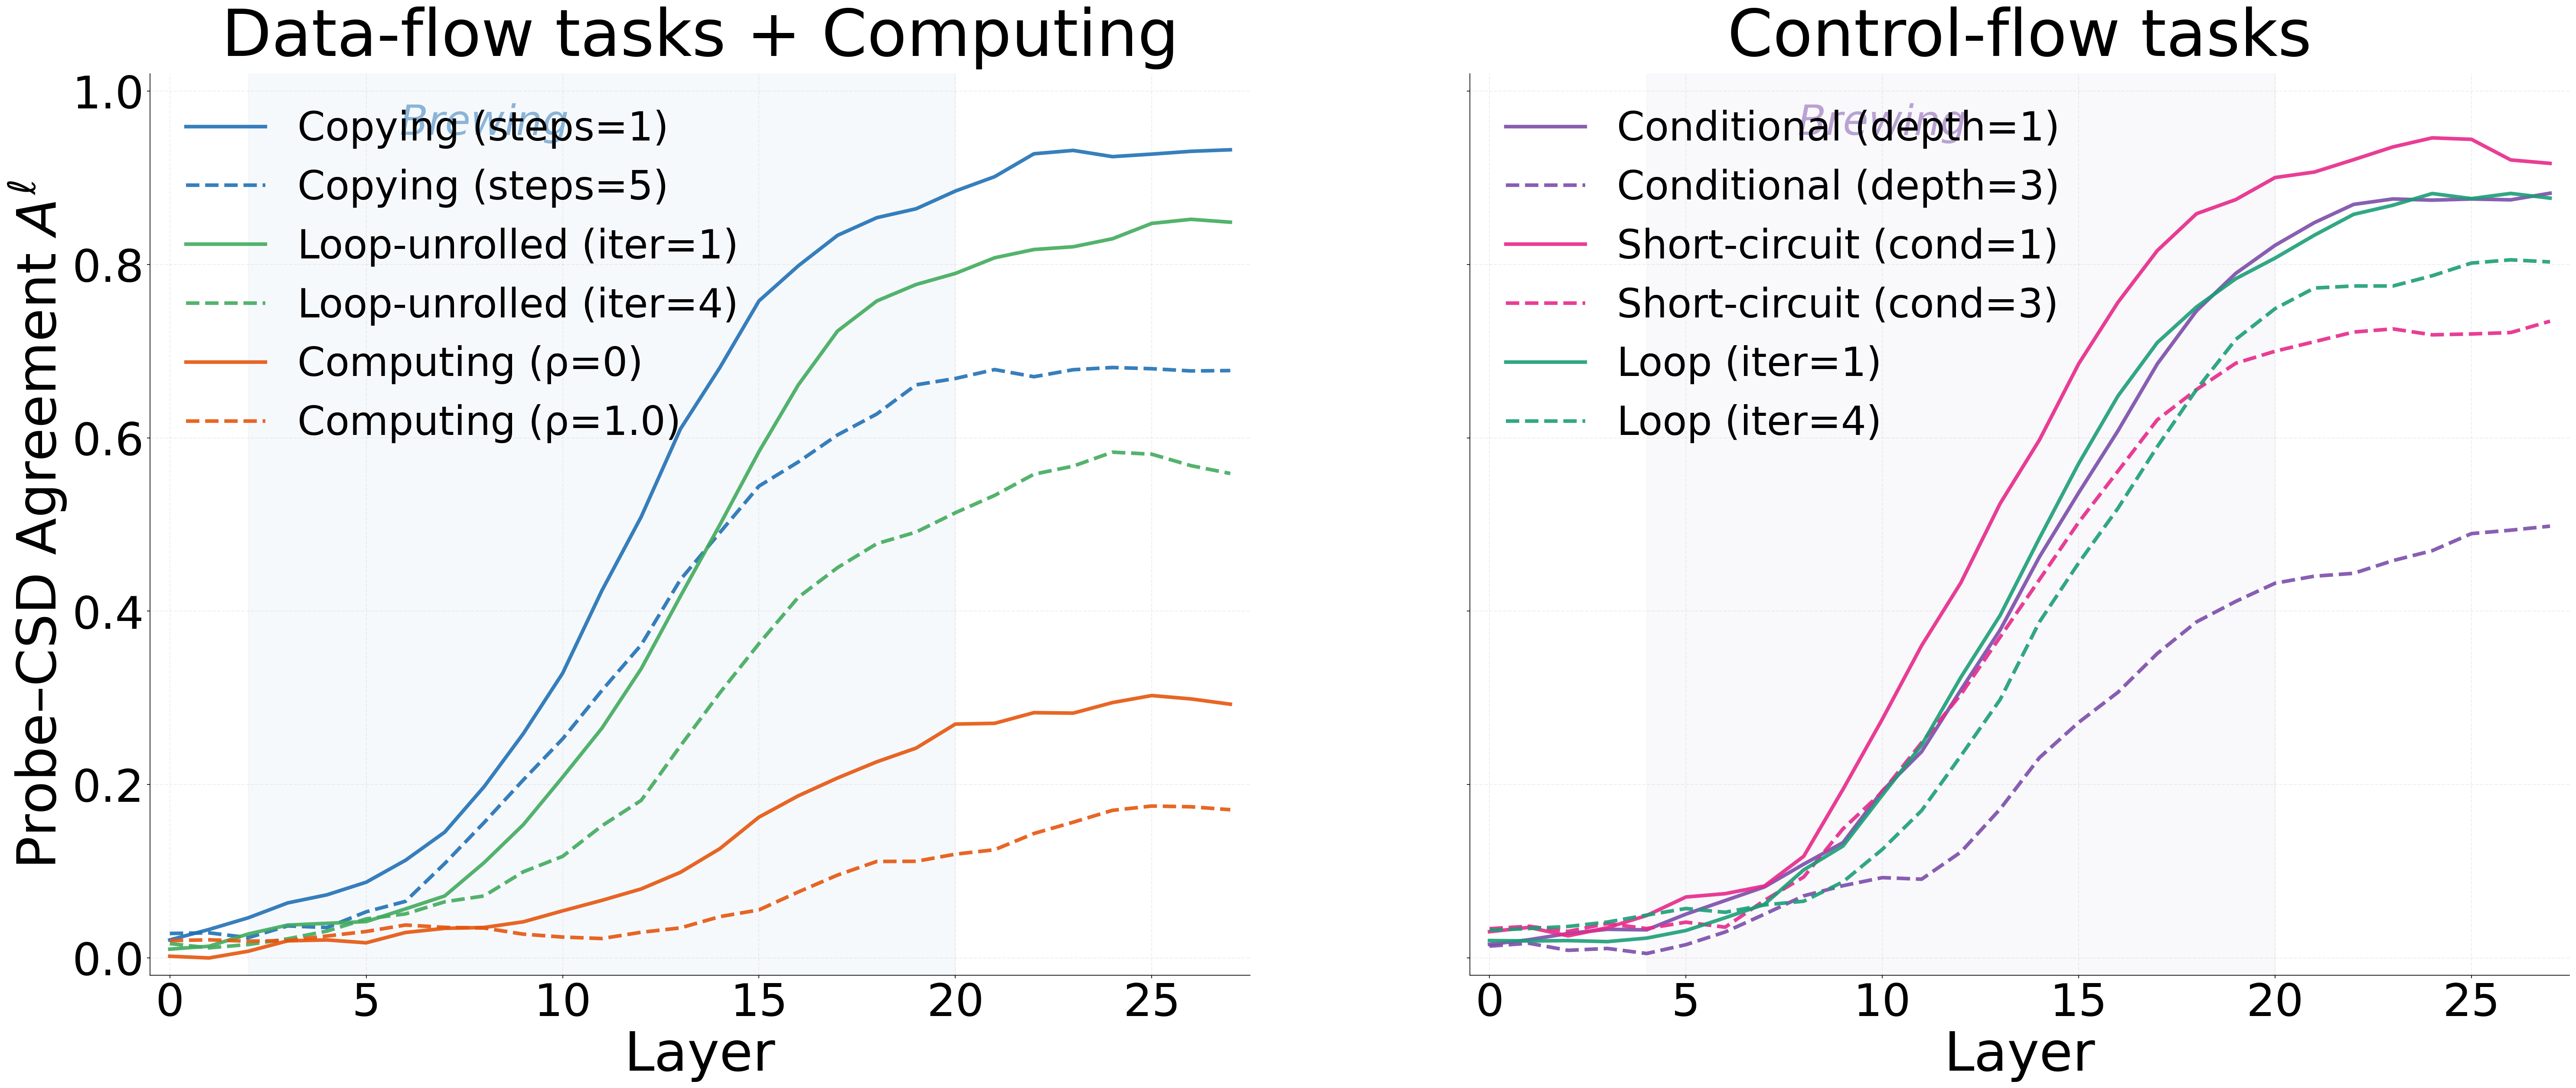
\includegraphics[width=\linewidth]{figures/appendix/G_brewing_dynamics_agreement.png}
\caption{Per-layer probe--CSD agreement $A^\ell$ trajectories for each task at selected difficulty levels. Agreement rises through the brewing phase and plateaus near FJC, with harder instances showing lower plateau values.}
\label{fig:app:brewing_agreement}
\end{figure}


% Appendix H: Cross-Architecture and Scaling
% Appendix H: Cross-Architecture and Scaling

\section{Cross-Architecture and Scaling}
\label{app:cross_architecture_and_scaling}

% 本节提供 §4.2 中跨模型、跨规模分析的完整数据。

\subsection{Coder vs.\ Base Paired Analysis}
\label{app:subsec:coder_vs_base}

% Qwen2.5-Coder 与 Qwen2.5 在各任务上的 outcome 分布对比。
% FJC 归一化层位的 Pearson 相关性数据与散点图。
% 预期效果：量化 code-specialized 训练对 outcome 分布的改善及对 FJC 位置的微弱影响。

% TODO: 插入 Coder vs Base 对比数据

\subsection{Scaling Trends}
\label{app:subsec:scaling_trends}

% 0.5B → 14B 的 outcome 分布变化趋势。
% Overprocessed 非单调趋势的详细数据。
% Normalized brewing duration 在不同规模间的稳定性数据。
% 预期效果：支撑 "capability changes but scaffold does not" 的 claim。

% TODO: 插入 scaling 趋势数据与图表

\subsection{Cross-Architecture Robustness}
\label{app:subsec:cross_architecture_robustness}

% CodeLlama/Llama 和 DeepSeek-Coder 上的 brewing 存在性与 outcome fingerprint 结构。
% 预期效果：证明 brewing-to-resolution 不是 Qwen 特有的，而是 transformer 处理代码的一般属性。

% TODO: 插入跨架构实验结果



\end{document}
